%%
%% This is file `sample-sigconf-biblatex.tex',
%% generated with the docstrip utility.
%%
%% The original source files were:
%%
%% samples.dtx  (with options: `sigconf-biblatex')
%% 
%% IMPORTANT NOTICE:
%% 
%% For the copyright see the source file.
%% 
%% Any modified versions of this file must be 
%% with new filenames distinct from sample-sigconf-biblatex.tex.
%% 
%% For distribution of the original source see the terms
%% for copying and modification in the file samples.dtx.
%% 
%% This generated file may be distributed as long as the
%% original source files, as listed above, are part of the
%% same distribution. (The sources need not necessarily be
%% in the same archive or directory.)
%%
%%
%% Commands for TeXCount
%TC:macro \cite [option:text,text]
%TC:macro \citep [option:text,text]
%TC:macro \citet [option:text,text]
%TC:envir table 0 1
%TC:envir table* 0 1
%TC:envir tabular [ignore] word
%TC:envir displaymath 0 word
%TC:envir math 0 word
%TC:envir comment 0 0
%%
%%
%% The first command in your LaTeX source must be the \documentclass
%% command.
%%
%% For submission and review of your manuscript please change the
%% command to \documentclass[manuscript, screen, review]{acmart}.
%%
%% When submitting camera ready or to TAPS, please change the command
%% to \documentclass[sigconf]{acmart} or whichever template is required
%% for your publication.
%%
%%
\documentclass[acmsmall,screen,review,anonymous]{acmart}


\usepackage{graphicx}
\usepackage{algorithm}
\usepackage{algpseudocode}
\usepackage{booktabs} 
\usepackage{threeparttable}
\usepackage{multirow}
\usepackage{enumitem}
\usepackage{colortbl}
\usepackage[most]{tcolorbox}
\usepackage{caption}
\usepackage[normalem]{ulem}
\usepackage{xcolor}
\usepackage{wrapfig}
\usepackage{url}

\usepackage{pifont}
\usepackage{booktabs}
\usepackage{cleveref}
\crefname{section}{§}{§§}
\Crefname{section}{§}{§§}

\newcommand{\mytodoblue}[1]{\textcolor{blue}{\ding{46}~{\sf}~#1}}
\newcommand{\mytodored}[1]{\textcolor{red}{\ding{46}~{\sf}~#1}}
\newcommand{\mytodogreen}[1]{\textcolor{mygreen}{\ding{46}~{\sf}~#1}}
\newcommand{\mytodoorange}[1]{\textcolor{orange}{\ding{46}~{\sf}~#1}}
\newcommand{\mytodocyan}[1]{\textcolor{cyan}{\ding{46}~{\sf}~#1}}
\newcommand{\mytodopink}[1]{\textcolor{purple}{\ding{46}~{\sf}~#1}}
\usepackage{pgffor}
\usepackage{pifont} % For checkmark and cross symbols

\usepackage{xcolor,pifont}

% 自定义彩色打勾和打叉命令
\newcommand{\cmark}{\textcolor{green!60!black}{\ding{51}}}   % 绿色打勾
\newcommand{\xmark}{\textcolor{red}{\ding{55}}}   % 红色打叉


% to show s or not
\newif\ifshowcomments
%\showcommentsfalse
\showcommentstrue
\ifshowcomments
\newcommand{\wu}[1]{\mytodored{[wu: #1]}}
\newcommand{\cp}[1]{\mytodored{[cp: #1]}}
%\newcommand{\zhang}[1]{\mytodoorange{[zhang: #1]}}
\newcommand{\lin}[1]{\mytodored{[lin: #1]}}
%\newcommand{\other}[1]{\mytodoblue{[other: #1]}}
\else
\newcommand{\wu}[1]{}
\newcommand{\cp}[1]{}
%\newcommand{\zhang}[1]{}
\newcommand{\lin}[1]{}
%\newcommand{\other}[1]{}
\fi

\newif\ifshowrevisioncomments
\showcommentsfalse
%\showrevisioncommentstrue
\showrevisioncommentsfalse
\ifshowrevisioncomments
\newcommand{\revision}[1]{\textcolor{blue}{{#1}}}
\newcommand{\deletion}[1]{\textcolor{red}{{\sout{#1}}}}
\else
\newcommand{\revision}[1]{#1}
\newcommand{\deletion}[1]{}
\fi


\newcommand{\toolname}{\textsc{OptSQL}}
\newcommand{\benchmark}{\textsc{EESQLBench}}
\newcommand{\tasknumber}{213}

\settopmatter{printacmref=false}
\setcopyright{none}
\renewcommand\footnotetextcopyrightpermission[1]{}
\pagestyle{plain}


% FSE 2027 Research Papers submission format:
% https://conf.researchr.org/track/fse-2027/fse-2027-papers
\acmConference[FSE '27]{35th ACM International Conference on the Foundations of Software Engineering}{July 12--16, 2027}{Shenzhen, China}
\acmYear{2027}
\copyrightyear{2027}
% Publication identifiers are assigned after acceptance.
\acmDOI{}
\acmISBN{}

\begin{document}
	\newtcolorbox{mybox}[2][]{
		colframe = black,
		colback  = gray!20,
		coltitle = black,
		left = 1mm,
		right = 1mm,
		top = 1mm,		bottom = 1mm,
		boxsep=5pt,
		arc=2mm,
		title=#2,
		#1
	}
	
	\title{OptSQL: A Meta-Cognitive Multi-Agent System for Efficiency-Oriented Text-to-SQL}
	
	
	\begin{abstract}
	Text-to-SQL aims to translate natural language questions into executable SQL queries. 
	Recent LLM-based systems have improved robustness through workflow-based generation, but they still rely on largely fixed pipelines, use feedback mainly for post-hoc repair, and focus primarily on correctness while overlooking query efficiency. 
	To address these limitations, we propose \toolname, a meta-cognitive multi-agent Text-to-SQL system that dynamically coordinates evidence construction, SQL generation, process-level reflection, and plan-aware optimization.
	A Meta-Cognitive Controller continuously observes the task state and database feedback to adapt workflow strategies, reflect on intermediate reasoning states, and perform execution- and plan-aware rewriting.
	We evaluate \toolname\ on \textsc{BIRD} and \textsc{EESQLBench}. 
	\toolname\ achieves the best EX of 73.29\% and AR@1 of 67.96\% on \textsc{BIRD}, and the best EX of 67.89\% and AR@1 of 50.59\% on \textsc{EESQLBench}. 
	These results show that meta-cognitive control improves the correctness and efficiency of Text-to-SQL systems.
\end{abstract}
	\maketitle
	\vspace{-2mm}
\section{Introduction}
\label{sec:intro}

% 第一段 ： Text-to-SQL 的背景
Text-to-SQL aims to translate natural language (NL) questions into executable SQL queries, enabling non-expert users to retrieve and analyze relational data without manually writing database programs~\cite{androutsopoulos1995natural,hendrix1978developing,popescu2003towards}. 
%Its importance has grown with increasingly large schemas, rich database contents, and diverse analytical tasks, motivating benchmarks such as \textsc{Spider}~\cite{yu2018spider}, \textsc{BIRD}~\cite{li2023can}. 
Recent LLM-based systems have achieved substantial progress through in-context learning, task decomposition and specialized agents, moving the field beyond single-shot generation toward workflow-based SQL construction~\cite{gao2023text,pourreza2023din,wang2023mac,talaei2024chess}.


% 第二段：现有 Text-to-SQL 典型工作流
\textbf{From Single-shot Generation to Agentic Workflows.}
As shown in Figure~\ref{fig:text-to-sql-pipeline}, modern Text-to-SQL systems typically organize SQL construction into three stages: pre-generation, generation, and post-generation.
In the pre-generation stage, the system grounds the natural language query in the database context through schema linking, value grounding, and information retrieval, thereby reducing the search space and enriching the input evidence~\cite{talaei2024chess,lewis2020retrieval,pham2026avsql,biswal2026agentsm}. 
In the generation stage, the model applies prompting strategies, query planning, and LLM-based reasoning to produce one or more candidate SQL queries~\cite{gao2023text,pourreza2023din,wang2023mac,chaturvedi2025sqlthought,heidari2025agentiql,yang2025marssql}. 
In the post-generation stage, these candidates are further checked and refined through execution validation, repair, and consistency- or ensemble-based selection~\cite{wang2022selfconsistency,pourreza2023din,yao2023react,wang2023mac,talaei2024chess,chaturvedi2025sqlthought,heidari2025agentiql,yang2025marssql}.
Compared with single-pass generation, such workflows are more robust because they decompose SQL construction into modular steps, strengthen database grounding, diversify candidate generation, and provide post-hoc opportunities for validation and refinement. 
%
%\textbf{Limitations of existing Text-to-SQL systems.} 
Despite these advances, existing Text-to-SQL systems still face three coupled limitations:

\begin{figure}[t]
	\centering
	\vspace{-3mm}
	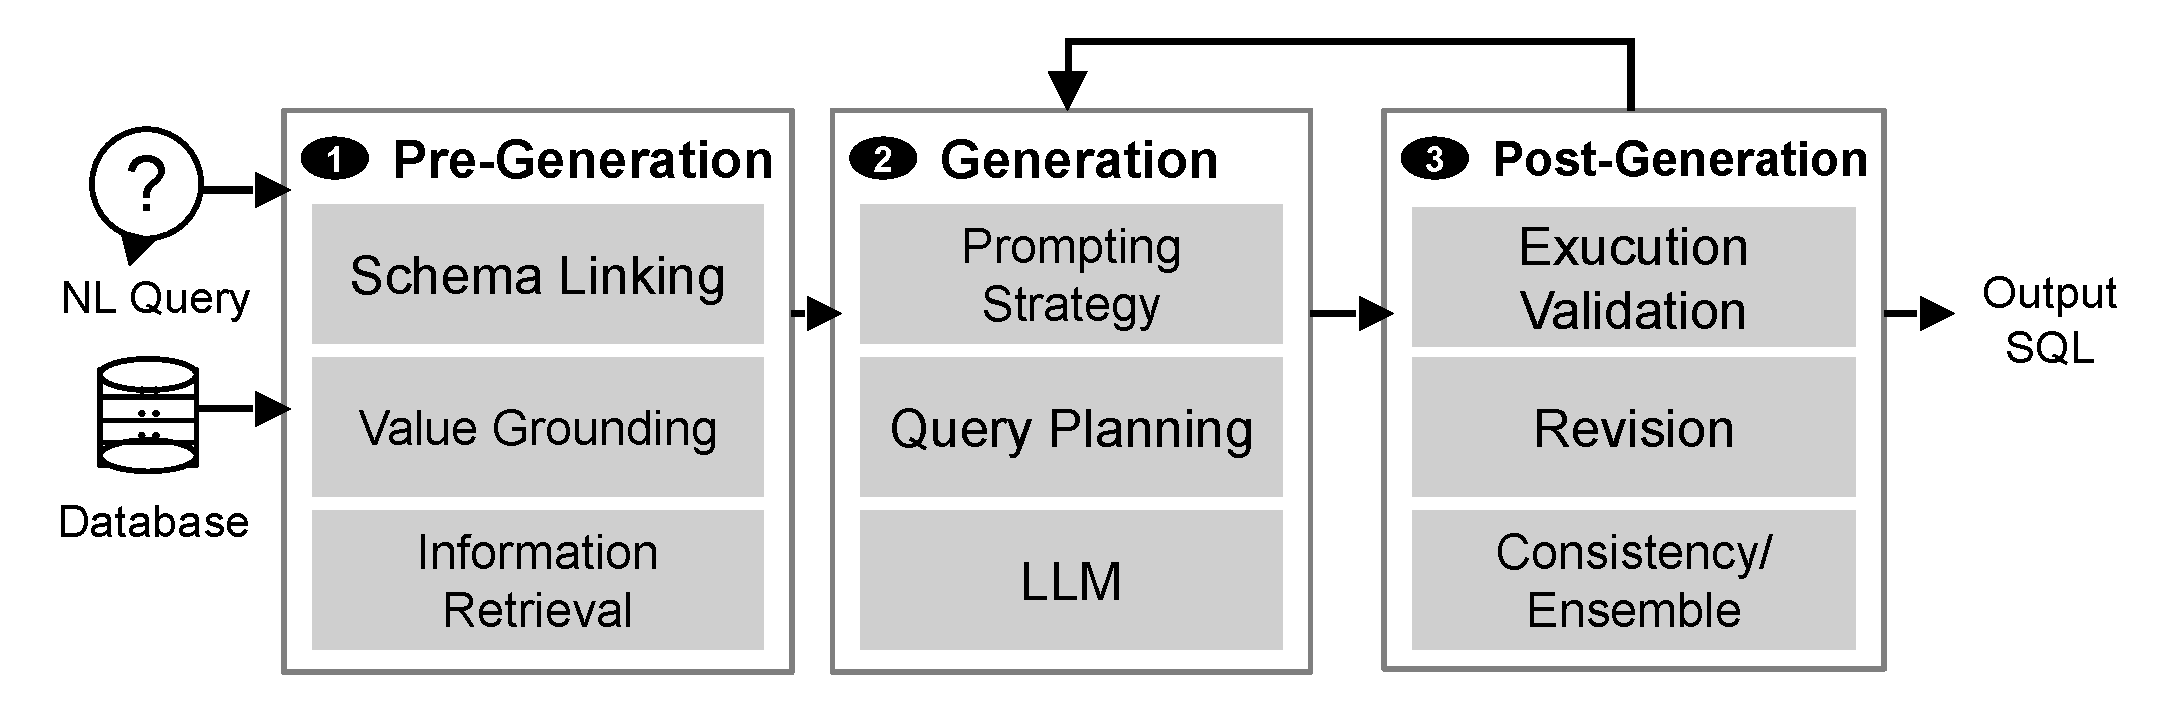
\includegraphics[width=0.95\linewidth]{./images/text-to-sql pipline.pdf} 
	\vspace{-4mm}
	\caption{\textbf{Overview of a typical Text-to-SQL pipeline, illustrating the Pre-Generation, Generation, and Post-Generation stages}}
	\label{fig:text-to-sql-pipeline}
	\vspace{-6mm}
\end{figure}

% 第3-5段，3个Limitations
%确实有一些工作开始做“自适应”，但多数只覆盖局部策略，而不是你这种结合环境感知、self-reflection、workflow/strategy selection 和 efficiency optimization 的 meta-cognitive controller。
%\textsc{CHESS} 会基于问题复杂度和上下文大小调整 schema pruning，但主要是 schema filtering 层面的自适应，不是全局 workflow selection。
%\textsc{QCMA-SQL} 明确做 question classification，并为不同复杂度问题调用不同 agents，比较接近“按难度选策略”。
%\textsc{OpenSearch-SQL} 提到 dynamic few-shot strategy 和 consistency alignment，更偏向 few-shot retrieval/selection 的局部自适应。
%还有一篇很新的 \textsc{SquRL} / “Beyond Static Pipelines” 直接批评 static pipeline，并通过强化学习学习动态 workflow；如果你后面 related work 要写，它可能需要重点区分。
%Although recent Text-to-SQL systems have introduced local adaptive mechanisms, such as difficulty-aware decomposition, adaptive schema pruning, dynamic demonstration retrieval, question-level agent routing, and even learned workflow policies, these adaptations are usually confined to specific stages of the pipeline.
%They provide limited support for jointly adapting the overall workflow, generation strategy, reflection behavior, and optimization effort according to the database environment, question difficulty, intermediate feedback, and execution efficiency.
% 我觉得需要讨论一下了
\textbf{L1: Limited Adaptation in Workflows and Strategy Selection.}
Many existing Text-to-SQL agents often predefine both the workflow structure and the strategy choices, where modules such as schema linking, few-shot retrieval, candidate generation, validation, and revision are applied in a largely fixed manner~\cite{gao2023text,pourreza2023din,wang2023mac,chaturvedi2025sqlthought,pham2026avsql}.
Although such designs improve robustness over single-shot generation, they offer limited support for adapting reasoning strategies to the database environment, question difficulty, or intermediate feedback.
This may misallocate reasoning effort: simple queries over intuitive schemas can incur unnecessary token and latency overhead, whereas difficult queries may require deeper grounding, candidate comparison, and additional validation or reflection.
This mismatch is illustrated by the different effects of domain-specific hints in \textsc{BIRD}~\cite{li2023can} dataset.
For an intuitive database such as \texttt{superhero}, where tables and columns are relatively descriptive, adding domain hints provides little additional benefit in our experiments.
In contrast, for a domain-heavy database such as \texttt{thrombosis\_prediction}, where terms such as \texttt{LDH} and gender-dependent uric-acid ranges require medical knowledge, the same hints improve accuracy from 20\% to nearly 50\%.
This contrast suggests that Text-to-SQL agents should adapt their grounding and generation strategies to the database environment, rather than applying the same strategy uniformly.

% 参考 MaCTG: Multi-Agent Collaborative Thought Graph for Automatic Programming
\textbf{L2: Post-hoc rather than Process-level Reflection.}
Feedback in many Text-to-SQL systems is mainly used after a candidate SQL has been generated, such as repairing execution errors, revising invalid queries, or selecting among completed candidates~\cite{pourreza2023din,wang2023mac,talaei2024chess,lei2024spider}.
Such feedback improves final-output validation, but provides limited support for monitoring and regulating the generation process itself.
In particular, the agent often lacks a controller that continuously tracks whether schema linking is reliable, whether candidate disagreement is increasing, whether repeated repairs are converging, or whether the current strategy should be changed.
As a result, early mistakes in schema linking, value grounding, or query planning may propagate into later steps and become cascading hallucinations.
Moreover, without global process supervision, local repair actions may fix surface-level execution errors while leaving the overall reasoning trajectory insufficiently grounded in the user question and database context.

\textbf{L3: Limited Awareness of Query Efficiency\footnote{Unless otherwise specified, efficiency in this paper refers to the execution efficiency of the generated SQL query, rather than the efficiency of LLM-based query generation.}.}
Most existing Text-to-SQL systems are primarily optimized for correctness: they aim to generate SQL queries whose execution results match the ground-truth answers~\cite{li2023resdsql,li2024codes,li2023graphix,rai2023improving,scholak2021picard}.
However, in practical database applications, a semantically correct SQL query is not necessarily efficient.
Equivalent SQL formulations may lead to very different execution costs due to variations in join orders, predicate placement, or aggregation strategies~\cite{chaudhuri1998overview,leis2015good,wang2022wetune}.
Yet, current Text-to-SQL systems mainly focus on executability and result consistency, rarely treating query plans, estimated costs, or bottleneck patterns as signals for rewriting generated SQL.
As a result, the final query may be correct but unnecessarily expensive, especially in enterprise settings with large schemas, large tables, and long multi-step analytical workflows~\cite{lin2026cracking,lei2024spider}.


% 第六段  key insights
\textbf{Key Insights: Meta-cognitive and Environment-aware Text-to-SQL.}
Inspired by enactive cognition and meta-cognition, we view Text-to-SQL not as a static translation from question and schema to SQL, but as an adaptive interaction process between the agent and the database environment~\cite{varela1991embodied,flavell1979metacognition}.
Enactive cognition suggests that understanding is shaped through interaction with the environment, while meta-cognition emphasizes the ability to monitor and regulate one's own reasoning process.
In the context of Text-to-SQL, this means that an agent should perceive database-specific signals, act by generating and rewriting SQL, observe feedback from execution and query plans, and adjust its strategy when uncertainty, failure, or inefficiency is detected.
These perspectives lead to three design objectives.
First, to address \textbf{L1}, the agent should perform \emph{environment-aware dynamic workflow adaptation}: it should select lightweight or deep workflows according to the perceived database environment, question complexity, and intermediate feedback, rather than applying the same strategy uniformly.
Second, to address \textbf{L2}, the agent should support \emph{process-level self-reflection and dynamic control}: it should monitor schema-linking reliability, candidate disagreement, repair convergence, and strategy suitability during generation, so that early mistakes can be corrected before they propagate.
Third, to address \textbf{L3}, the agent should enable \emph{execution- and plan-aware SQL optimization}: it should use query plans, cost signals, semantic validation, and reusable rewrite knowledge to improve query efficiency while preserving correctness.

% 第七段 approach
\textbf{Approach.} 
To realize these objectives, we propose \toolname, a meta-cognitive multi-agent system for efficiency-oriented Text-to-SQL.
At the core of \toolname\ is a Meta-Cognitive Controller that maintains a task-level state in working memory, observes intermediate feedback, and dynamically decides which agent actions should be invoked next.
Under its control, the Generation Phase constructs executable and semantically plausible initial SQL candidates through evidence-guided schema filtering and multi-strategy SQL generation.
When further efficiency improvement is needed, the Optimization Loop analyzes query plans, identifies bottleneck patterns, rewrites inefficient SQL formulations, and validates both semantic consistency and cost reduction.
Finally, a Memory Engine and Tool Infrastructure support database grounding, execution analysis, retrieval of reusable optimization experience, and updates to the long-term Auto-Evaluation Knowledge Base (AEKB) after successful rewrites.

% 第八段 evaluation
\textbf{Evaluation.}
We evaluate \toolname\ on two complementary benchmarks, \textsc{BIRD}~\cite{li2023can} and \textsc{EESQLBench}~\cite{lin2026cracking}, covering both general cross-domain Text-to-SQL capability and efficiency-oriented SQL generation.
We compare \toolname\ with fine-tuning-based methods, prompting-based methods, and agentic Text-to-SQL workflows under multiple backbone LLMs.
The results show that \toolname\ achieves the best or highly competitive performance across correctness- and efficiency-oriented metrics, including EX, VES, CR, AR@0.8, and AR@1 (see Section~\ref{sec:evaluation}).
In particular, \toolname\ achieves the best EX of 73.29\% and AR@1 of 67.96\% on \textsc{BIRD}, and the best EX of 67.89\% and AR@1 of 50.59\% on \textsc{EESQLBench}.
These results show that \toolname\ effectively bridges semantic correctness and efficiency, validating the benefits of meta-cognitive control for practical Text-to-SQL systems.

% 第九段 contributions
In summary, this paper makes the following contributions:
\begin{itemize}[leftmargin=10pt]	
	
	\item We identify three key limitations of existing Text-to-SQL systems: limited workflow adaptation, post-hoc reflection, and insufficient awareness of query efficiency.
	
	\item We propose \toolname, a meta-cognitive multi-agent system that dynamically coordinates evidence construction, SQL generation, process-level reflection, and plan-aware optimization.
	
	\item We evaluate \toolname\ on \textsc{BIRD} and \textsc{EESQLBench}, showing consistent improvements over prompting-based, fine-tuning-based, and agentic baselines.
\end{itemize}

	\vspace{-2mm}
\section{Motivation}
\label{sec:preliminaries}
% 减少公式之间的间距
\begingroup
\setlength{\abovedisplayskip}{3pt}
\setlength{\belowdisplayskip}{3pt}
\setlength{\abovedisplayshortskip}{2pt}
\setlength{\belowdisplayshortskip}{2pt}
\setlength{\jot}{2pt}

\subsection{Task Formulation}
Traditional Text-to-SQL aims to translate an NL question $x$ into an executable SQL query $q$ over a database environment $\mathcal{D}$.
Given a ground-truth query $q^*$, the standard objective is to generate a query whose execution result matches that of $q^*$:
\[
f_\theta(x, \mathcal{D}) \rightarrow q,
\quad
\text{s.t.} \quad
\text{Exec}(q, \mathcal{D}) = \text{Exec}(q^*, \mathcal{D}),
\]
where $f_\theta$ denotes a Text-to-SQL system parameterized by $\theta$, $\mathcal{D}$ denotes the database environment including schema, data, indexes, and statistics, and $\text{Exec}(q, \mathcal{D})$ denotes the result of executing $q$ on $\mathcal{D}$.

However, this formulation focuses mainly on semantic correctness and does not explicitly consider query efficiency.
In practice, multiple semantically equivalent SQL queries may produce the same result but incur substantially different execution costs due to join order, predicate placement, aggregation strategy, or index utilization.
We therefore formulate \textbf{Efficiency-Oriented Text-to-SQL}, where the goal is to generate a query that is both semantically correct and efficient.
Given an NL question $x$ and a database environment $\mathcal{D}$, the goal is to generate a SQL query $q_{\text{opt}}$ satisfying:
\[
\begin{aligned}
	q_{\mathrm{opt}}
	&= \arg\min_{q \in \mathcal{Q}_{\mathrm{corr}}(x,\mathcal{D})}
	\; \text{Cost}(q,\mathcal{D}), \\
	\mathcal{Q}_{\mathrm{corr}}(x,\mathcal{D})
	&= \{q \in \mathcal{Q}(x,\mathcal{D}) \mid \text{Exec}(q,\mathcal{D}) = \text{Exec}(q^*,\mathcal{D})\},
\end{aligned}
\]
where $\mathcal{Q}_{\mathrm{corr}}(x,\mathcal{D})$ denotes the subset of candidates that are semantically correct with respect to $q^*$.
$\text{Cost}(q, \mathcal{D})$ represents the estimated or actual execution cost of query $q$ on $\mathcal{D}$.
Intuitively, the model should not only ensure that $q_{\text{opt}}$ yields correct results but also that it achieves minimal execution time or resource consumption under the same semantic constraints. 

\revision{
	The minimization above specifies the ideal task objective.
	The reference query $q^*$ supplies the expected result for correctness evaluation and is not assumed to be a minimizer of $\text{Cost}$.
	Our research question is whether and how adaptive agent orchestration guided by execution and query-plan feedback can improve the efficiency of generated SQL while preserving correctness.
	Operationally, \toolname\ explores and validates a finite set of candidates, and its effectiveness is assessed through empirical improvements over baseline systems and comparisons with reference queries, without claiming exhaustive search or global optimality.
}

\vspace{-2mm}
\subsection{Design Objective}
Existing Text-to-SQL systems are typically static pipelines that decompose SQL construction into pre-defined stages, including pre-generation, generation, and post-generation validation. 
While such designs improve robustness compared to single-pass generation, they lack the ability to dynamically adapt their reasoning process to different database environments, query difficulties, and intermediate execution feedback.

\textbf{Beyond Static Pipelines: A Meta-Cognitive Multi-Agent Perspective.}
Inspired by enactive cognition and meta-cognitive theory, we reformulate Text-to-SQL as a dynamic interaction process between an intelligent system and the database environment~\cite{varela1991embodied,flavell1979metacognition}.
Enactive cognition emphasizes that intelligence emerges through continuous interaction with the environment, while meta-cognition enables the system to monitor, regulate, and adapt its own reasoning process.
Based on these principles, we propose a Meta-Cognitive Multi-Agent Text-to-SQL System, where a central Meta-Cognitive Controller dynamically orchestrates a set of specialized agents (actions) under different execution contexts.
Instead of a fixed pipeline, all stages in Text-to-SQL are decomposed into reusable and composable actions, which are invoked online based on the current state of the problem and environment feedback.
This design establishes a unified closed-loop system in which a Meta-Cognitive Controller coordinates planning, execution, evaluation, and optimization over SQL programs based on continuous database feedback.

\textbf{Key Design Principles.}
%Principle 1: task memory → decide what action to invoke next
%Principle 2: task memory → diagnose whether current reasoning path is unreliable and needs correction
\textbf{(1) Environment-aware Dynamic Workflow Adaptation.}
The Meta-Cognitive Controller continuously observes the evolving task state, such as database environment, question complexity, candidate behaviors and dynamically decides which actions should be invoked next.
For example, for simple queries over well-structured schemas (e.g., single-table filtering), the controller may directly invoke a lightweight generation path using few-shot prompting.
In contrast, for complex analytical queries (e.g., multi-join or domain-specific reasoning), the controller activates a deeper workflow that includes multi-candidate generation, iterative refinement, and optimization loops.
This adaptive strategy selection avoids over- or under-utilization of reasoning resources.

\textbf{(2) Process-level Self-Reflection and Dynamic Control.}
Unlike conventional post-hoc validation approaches, our system enables continuous monitoring of intermediate reasoning states during SQL generation.
The Meta-Cognitive Controller uses the recorded task trace to diagnose whether the current reasoning trajectory is reliable, converging, and sufficiently grounded.
For example, when schema or value evidence is insufficient, the controller may request additional evidence construction through reverse schema linking, value-grounded schema linking, or relational completion.
Similarly, if repeated optimization iterations fail to reduce execution cost, the controller may terminate the current loop and switch to a different reasoning configuration.
This enables closed-loop control over the entire reasoning trajectory.

\textbf{(3) Execution- and Plan-aware Optimization via Feedback-driven Rewriting.}
Beyond generating semantically correct SQL, the system treats execution efficiency as an objective.
Execution results, query plans, and cost estimates are used as feedback signals to reveal whether an initially correct query may still be inefficient.
When such feedback indicates potential performance bottlenecks, the system can refine the SQL through feedback-driven rewriting while preserving its intended semantics.
Optimization is not treated as an isolated one-shot action.
The system accumulates validated optimization experience from previous interactions with the database environment, enabling future decisions to be guided not only by static rules but also by reusable execution-aware experience.
In this way, SQL optimization becomes a closed-loop process in which database feedback continuously informs rewriting, validation, and future strategy selection.


\endgroup

%	\section{EESQLBench}
\label{sec:EESQLBench}

In this section, we introduce the construction of \benchmark , the first benchmark for evaluating Efficiency-Oriented Text-to-SQL tasks.
Figure \ref{fig:overview} illustrates the entire process involved in building our benchmark.
Starting from real-world databases, we enhance database schemas and data instances to expose performance-sensitive behaviors, and generate   complex SQL queries that admit substantial optimization opportunities.
For each generated query, we further curate a semantically equivalent but efficiency-optimized canonical SQL via automated rewriting and expert refinement, and align it with a natural language (NL) question.
More details will be introduced in the following subsections.

\subsection{Benchmark Construction}
% Implementation

\begin{figure}[t]
	\centering
	\includegraphics[width=0.9\linewidth]{./images/Overview.pdf} 
	\vspace{-5mm}
	\caption{\textbf{Overview of \benchmark\ Construction Pipeline}}
	\label{fig:overview}
	\vspace{-5mm}
\end{figure}

\subsubsection{Database Preparation.}
We prepare the databases of \benchmark\ by building upon real-world relational databases collected from the \textsc{BIRD}~\cite{li2023can} benchmark.
We choose \textsc{BIRD}~\cite{li2023can} because it covers cross-domain scenarios spanning diverse application areas, including e-commerce, finance, and healthcare, and provides large-scale tables derived from real-world data with rich relational structures and realistic data distributions.
Based on these databases, we enhance the original schemas to better support efficiency-oriented evaluation.
% 修复外键
In particular, we explicitly repair missing or implicit foreign-key relationships, which enables multiple alternative join paths among related tables and allows semantically equivalent SQL queries to be expressed in structurally different forms.
% 随机添加索引
We further apply mixed indexing strategies by randomly indexing a subset of foreign-key and attribute columns, so that different join orders and access paths can lead to distinct execution plans. 
% 插入数值和噪声数据，数据分布
At the instance level, we enlarge the databases by systematically inserting additional rows into existing tables while strictly preserving the original schemas, data types, and foreign-key constraints.
For each table, new tuples are generated by sampling valid key values from referenced tables and duplicating existing records with controlled variations on non-key attributes.
We explicitly control value frequencies for selected predicate-relevant attributes by making some values significantly more frequent than others, thereby introducing skewed data distributions that amplify efficiency differences among semantically equivalent queries.


\subsubsection{Complexity-Aware Query Generation.}
After preparing databases, we synthesize SQL queries that are both structurally complex and optimization-sensitive.
We adopt a reverse construction strategy: instead of starting from NL and hoping a generator produces sufficiently challenging SQL, we first generate complex SQL candidates and then align them with NL questions.
%Our design is inspired by DBMS fuzzing, which is effective at exploring a wide spectrum of query structures (e.g., deep nesting, multi-join chains, and aggregation patterns) that can expose optimizer behaviors.
%However, directly using off-the-shelf fuzzers often yields many ill-typed, semantically invalid, or practically meaningless queries, while directly prompting an LLM tends to produce overly ``clean'' and repetitive SQL due to pretraining biases.
%This means LLM-generated queries often exhibit limited structural diversity, favoring simple join patterns and shallow nesting that provide few opportunities for efficiency-sensitive analysis.
Our design is inspired by DBMS fuzzing, which can explore a wide spectrum of query structures (e.g., deep nesting, multi-join chains, and aggregation patterns) that are useful for stress-testing optimizer behavior.
However, off-the-shelf fuzzers are not directly applicable: they often produce ill-typed, semantically invalid, or practically meaningless queries.
On the other hand, prompting an LLM can improve semantic plausibility and executability, but the generated SQL is often overly ``clean'' and repetitive due to pretraining biases, favoring simple join patterns and shallow nesting.
As a result, neither approach alone can simultaneously provide high structural diversity and semantic validity.
To balance these two objectives, we introduce a \emph{SQL Sketch} mechanism that decouples \emph{query structure} from \emph{schema-specific semantics}.
As illustrated in Figure~\ref{fig:sql template}, query generation proceeds in two stages: (i) grammar-based SQL sketch generation, which generates the high-level relational structure of a query, and (ii) LLM-based instantiation, which binds schema-dependent elements under explicit constraints.

\begin{figure}[t]
	\centering
	\includegraphics[width=1\linewidth]{./images/SQL template.pdf} 
	\vspace{-8mm}
	\caption{\textbf{Two-Stage Query Generation via Grammar-Based SQL Sketching and LLM-Based Instantiation}}
	\label{fig:sql template}
	\vspace{-7mm}
\end{figure}

\textbf{(1) Grammar-Based SQL Sketch Generation.}
We firstly generate SQL sketches by sampling from a context-free grammar that specifies optimization-sensitive query structures.
We implement this grammar as shown in Figure \ref{fig:sql template} and use \textsc{go-randgen}~\cite{go-randgen} as a grammar-based generator to derive grammar-valid sketches, covering patterns such as multi-table joins, nested subqueries, common table expressions (CTEs), and aggregations with \texttt{HAVING} clauses.
By construction, each sketch fixes the high-level composition and nesting of relational operators, while abstracting away schema-specific details.
Concretely, schema-dependent elements—including table names, column references, join predicates, and literal constants—are replaced with typed placeholders (denoted by identifiers prefixed with an underscore, e.g., \texttt{\_table}, \texttt{\_cte\_table}, \texttt{\_column}, \texttt{\_agg\_func}, \texttt{\_const}).
This sketch-based design ensures structural correctness and diversity at the query level, while deferring schema binding and semantic instantiation to a later stage.

\textbf{(2) LLM-based Query Instantiation.}
Given a target database, we prompt an LLM to instantiate each sketch by filling placeholders with concrete tables, columns, predicates, and values.
To improve semantic plausibility and controllability, the instantiation prompt includes the following components:
\begin{itemize}[leftmargin=10pt]
	\item \textbf{Task Instruction:} Instructs the LLM to fill the provided SQL sketch into an executable query that corresponds to a meaningful analysis intent, rather than producing arbitrary or trivial SQL.
	\item \textbf{Database Schema:} Provides the full \texttt{CREATE TABLE} statements (table names, columns, types, primary keys, and foreign keys) so that the LLM can select type-consistent columns and produce join conditions aligned with the schema constraints.
	\item \textbf{Database Values:} Samples representative values for a few columns (e.g., categorical values, typical timestamps, common IDs) to ground predicate generation, reducing ill-formed conditions (e.g., comparing strings to numeric columns) and improving contextual relevance.
%	\item \textbf{Column Selection Constraint:} Specifies the target number of output columns (e.g., sampled from a small-biased distribution) so that the generated query returns a concise result schema, consistent with common user-facing analytical questions that focus on a few key attributes.
	\item \textbf{Few-shot Examples:} Provides a small number of example queries following the same formatting and style, helping the LLM adhere to the desired SQL conventions (e.g., aliasing, indentation, and aggregation style).
\end{itemize}
The LLM is explicitly instructed to satisfy typing constraints and foreign-key connectivity when instantiating placeholders, producing executable SQL candidates.

Finally, we validate each instantiated query through execution.
Queries that fail to parse, violate schema constraints, or produce empty results are discarded.
%Only queries that execute successfully and exhibit non-trivial intermediate data processing are retained.
This process results in a large pool of complex and semantically meaningful SQL queries that admit substantial optimization opportunities, which are used in subsequent canonicalization and question alignment.

\subsubsection{Efficient Query Construction.}
For each synthesized SQL query, our goal is to construct a semantically equivalent but execution-efficient canonical query that represents expert-level optimization.
To this end, we adopt a two-stage optimization pipeline that combines automated query rewriting with expert refinement, and explicitly annotate the applied optimization types.
As a first step, we apply an automated query rewriting procedure to identify candidate efficiency improvements.
Specifically, we leverage \textsc{WeTune}~\cite{wang2022wetune}, a rule-based query rewriting framework, to generate semantically equivalent query variants through systematic application of rewriting rules.
For each original query, we evaluate the rewritten variants and retain those that exhibit reduced execution cost.
Building upon the automatically rewritten candidates, database experts further refine the queries to produce a final optimized canonical SQL.
% 专家的选择
In this project, we engage three full-time Text-to-SQL experts, all of whom are Ph.D. students with formal training in hands-on experience in SQL optimization and query tuning. 
The entire expert refinement process for all queries takes approximately 80 person-hours in total.
During this stage, experts manually inspect query structures and execution plans, and apply domain knowledge to introduce deeper optimizations that are difficult to fully capture by rule-based systems.
In addition, we explicitly annotate the primary optimization types applied to each query pair.
Each query pair is labeled with one or more optimization categories indicating where efficiency gains are achieved, such as \emph{join reordering}, \emph{predicate pushdown}, \emph{subquery elimination}, and \emph{aggregation rewriting}.
For example, if an optimized query achieves lower execution cost by pushing a filtering predicate from an outer query into an inner subquery before aggregation, it is annotated with \emph{predicate pushdown}.
These annotations enable fine-grained analysis of Text-to-SQL systems’ optimization capabilities.


\subsubsection{Natural Language Question Alignment.}
After constructing pairs of semantically equivalent original and optimized SQL queries, we align them with NL questions that faithfully capture the underlying analytical intent.
The key design principle of this stage is to ensure fairness: each NL question should reflect the high-level user intent of the query, without encoding any SQL-specific structures or optimization decisions.
To achieve this, we generate NL questions based on the shared semantics of each original–optimized query pair, rather than directly mirroring either concrete SQL formulation.
Specifically, we adopt a back-translation strategy in which an LLM is prompted to translate a given SQL query into a concise and natural NL question.
Importantly, the prompt provides both the original SQL and the optimized canonical SQL as semantic references, and explicitly instructs the model to generate a question that is simultaneously satisfied by both queries.
Concretely, the prompt is constructed with the following components:
\begin{itemize}[leftmargin=10pt]
	\item \textbf{Task Instruction.} 
	The model is instructed to generate a NL question that describes the analytical goal of the queries—i.e., what information is requested—rather than how the result is computed.
	
	\item \textbf{Dual Semantic References.} 
	Both the original SQL query and its optimized canonical counterpart are provided as semantic references.
	The model is instructed to infer the common analytical intent underlying the two queries and generate a single NL question that is valid for both, treating the SQLs as black-box specifications of the result.
	
	\item \textbf{Implementation Abstraction Constraint.} 
	The prompt explicitly prohibits mentioning SQL-specific constructs, such as joins, subqueries, aggregation operators, execution order, or optimization strategies, and requires the question to be phrased in natural, user-centric terms.
	
	\item \textbf{Semantic Equivalence Constraint.} 
	The generated question must remain answerable by any semantically equivalent SQL formulation, ensuring neutrality with respect to different query structures and execution strategies.
\end{itemize}
Following generation, all NL questions undergo a human verification and refinement step.
Three experts check each question for semantic alignment with both SQL variants, clarity, and naturalness, and revise ambiguous or overly verbose descriptions when necessary.
As a result, each NL question in \benchmark\ represents a realistic, user-facing query intent, and that can be correctly answered by multiple semantically equivalent SQL queries.
This alignment strategy enables \benchmark\ to simultaneously evaluate (i) semantic correctness, by checking whether a model-generated SQL answers the NL question correctly, and (ii) efficiency awareness, by comparing the execution efficiency of the generated SQL against the expert-optimized canonical query.

\subsubsection{Quality Control and Annotations.}
\label{subsubsec:quality control}
In the final stage, we conduct quality control for each Text-to-SQL task to ensure the correctness, consistency, and reliability of the benchmark.
This stage consists of semantic consistency verification and task difficulty annotation.

\textbf{(1) Semantic consistency verification.}
We first verify the semantic consistency of each task across both SQL queries and the corresponding NL question.
Specifically, we check that the original SQL query and the optimized SQL query are semantically equivalent by executing them under the same database configuration and comparing their result sets.
Meanwhile, we require the optimized query to consistently achieve lower execution cost, ensuring the presence of a genuine and stable efficiency gap.
We further verify that the NL question can be correctly answered by both SQL queries, confirming that it accurately captures their shared analytical intent.

\textbf{(2) Task difficulty annotation.}
After passing semantic consistency verification, we annotate the difficulty of each Text-to-SQL instance using a rule-based human scoring scheme along three complementary dimensions:
\begin{itemize}[leftmargin=10pt]
	\item \textbf{Schema Complexity:} the number of involved tables, join relationships, and foreign-key dependencies;
	\item \textbf{Question Understanding:} the presence of multiple conditions, implicit constraints, or required reasoning in the NL question;
	\item \textbf{SQL Complexity:} the structural and operator-level complexity of the query, such as subqueries, aggregations, \texttt{HAVING} clauses, and CTEs.
	%	SQL 复杂性是根据 Optimized 的判断的
\end{itemize}
Each dimension is graded according to predefined criteria specified in the annotation guidelines~\cite{eesqlbench_guidelines}, and the final difficulty label (e.g., Simple, Medium, or Hard) is determined by aggregating the scores across all dimensions.

All verification and annotation procedures are conducted by three domain experts.
Two experts independently evaluate each instance following a unified guideline, and disagreements are resolved by a third expert acting as an adjudicator.
We measure inter-annotator agreement using Cohen’s kappa coefficient, obtaining an overall kappa score of 0.92, which indicates high annotation consistency and reliable quality.
As a result, each task in \benchmark\ is accompanied by structured annotations, including the database context, paired original and optimized SQL queries, a shared NL question, explicit optimization-type labels, and a difficulty level.
These annotations provide a reliable foundation for analyzing both semantic correctness and optimization awareness of Text-to-SQL systems.

\subsection{Statistics}

\begin{wrapfigure}{r}{0.45\textwidth}
	\vspace{-14mm}
	\centering
	\includegraphics[width=0.45\textwidth]{./images/DB Complexity.pdf}
	\vspace{-5mm}
	\caption{\textbf{Distributions of Database Size in \benchmark\ (Log Scale)}}
	\label{fig:statistics}
	\vspace{-4mm}
\end{wrapfigure}
We present a statistical analysis of \benchmark\ and compare it with representative Text-to-SQL benchmarks in Table~\ref{tab:text2sql_stats}.
\benchmark\ is constructed on MySQL as the execution backend.
Overall, \benchmark\ contains \tasknumber\ Text-to-SQL tasks over 69 real-world databases.
All tasks are manually curated and paired with expert-optimized canonical SQL queries, enabling direct efficiency comparison between model-generated SQL and expert-level solutions.
Following a unified guideline (Section~\ref{subsubsec:quality control}), we further label each task with a difficulty level, resulting in 55 Simple, 85 Medium, and 73 Hard tasks.

%Figure~\ref{fig:statistics} shows the distribution of database sizes in \benchmark\ (log scale).
Figure~\ref{fig:statistics} shows the distribution of database sizes in \benchmark\ on a log scale; for completeness, we provide a detailed breakdown of record counts in our online documentation~\cite{eesqlbench_database_size}.
\benchmark\ covers databases with highly heterogeneous instance scales, spanning from 148kB to 4.4 GB.
In addition, \benchmark\ is explicitly designed to be efficiency-aware at three levels.
At the \emph{schema level}, each database contains 7.75 tables on average (and up to 65), with repaired foreign-key relationships that enable multiple semantically equivalent join paths.
At the \emph{instance level}, each database contains 3,432,599 records on average, and we further introduce controlled table-scale imbalance and value-frequency skew to amplify cost gaps among semantically equivalent queries.
At the \emph{query level}, each task involves 3.55 tables on average (up to 11) and 2.88 subqueries on average (up to 8), resulting in a substantial portion of multi-join and nested queries that admit non-trivial optimization opportunities.



\section{Efficiency-Oriented Evaluation Metrics}
\label{sec:metrics}
%1、EX
%2、在EX通过的基础上统计 Execution Time 、Actual Rows？
%3、计算与人工解的比值？

Evaluating Efficiency-Oriented Text-to-SQL requires metrics that not only assess semantic correctness but also reliably quantify query execution efficiency. 
While execution latency is a natural indicator of efficiency, it is highly sensitive to external factors, making it unstable and difficult to reproduce. 
Therefore, we adopt query-plan-based cost metrics, which provide a more stable proxy for intrinsic query efficiency.

\paragraph{Semantic Correctness.}
We first evaluate whether a generated query $\hat{q}$ is semantically equivalent to the canonical query $q^*$.
Following prior works~\cite{yu2018spider,li2023can}, semantic equivalence is determined by comparing execution results:
\[
\mathbf{1}(q^*, \hat{q}) =
\begin{cases}
	1, & \text{if } \text{Exec}(\hat{q}, \mathcal{S}) = \text{Exec}(q^*, \mathcal{S}), \\
	0, & \text{otherwise}.
\end{cases}
\]
Efficiency-related metrics are computed only on semantically correct queries (i.e., those with $\mathbf{1}(q^*, \hat{q}) = 1$), ensuring that efficiency evaluation is not confounded by incorrect query semantics.

\paragraph{\textbf{Cost Reachability (CR)}}
To measure a model-generated query's proximity to expert-level efficiency,
we introduce \emph{Cost Reachability (CR)}.
For each semantically correct query pair $(q^*, \hat{q})$, we define:
\[
CR_n = \frac{\text{Cost}(q^*, \mathcal{S})}{\text{Cost}(\hat{q}, \mathcal{S})},
\]
where $\text{Cost}(q, \mathcal{S})$ denotes the execution cost of query $q$ on schema $\mathcal{S}$, 
obtained from the query execution plan.
A larger $CR_n$ indicates that the generated query $\hat{q}$ is more efficient relative to the canonical solution $q^*$, 
while $CR_n < 1$ implies inferior efficiency.

To mitigate the influence of extreme outliers, we follow prior cost-based evaluation practices~\cite{li2023can} and apply a square-root transformation to obtain a stabilized score:
\[
R_n = \sqrt{CR_n}.
\]
The overall Cost Reachability is then computed as:
\[
CR_{\text{avg}} =
\frac{1}{\sum_{n=1}^{N} \mathbf{1}(q^*_n, \hat{q}_n)}
\sum_{n=1}^{N} \mathbf{1}(q^*_n, \hat{q}_n) \cdot R_n,
\]
where $N$ is the total number of evaluation instances. For brevity, we use CR to refer to the aggregated score $CR_{\text{avg}}$ in the remainder of the paper.

\paragraph{\textbf{Acceptable Reachability at $k$ (AR@$k$).}}
While $CR_{\text{avg}}$ characterizes the efficiency gap \emph{conditioned on semantic correctness}, it does not reflect how often a model produces queries that are both correct and practically efficient.
To capture this end-to-end utility, we define \emph{Acceptable Reachability at $k$} (AR@$k$) as:
\[
AR@k =
\frac{1}{N}
\sum_{n=1}^{N} \mathbf{1}(q^*_n, \hat{q}_n) \cdot \mathbf{1}(CR_n \ge k),
\]
where $k \in (0,1]$ is a user-defined threshold.
Intuitively, AR@$k$ measures the fraction of all test instances for which the generated SQL is semantically correct and its execution cost does not exceed $1/k$ times that of the canonical solution.
For example, $k=0.5$ corresponds to accepting queries that are at most twice as expensive as the expert-optimized SQL, while $k=1.0$ only counts queries whose execution cost is no higher than the canonical solution (i.e., at least as efficient as the expert-optimized SQL).

Together, CR and AR@$k$ provide complementary perspectives on efficiency:
CR measures \emph{how close} a model can get to expert-level efficiency on average (given correctness),
while AR@$k$ measures \emph{how often} it produces SQL that is both correct and meets a practical efficiency threshold.


	\vspace{-2mm}
\section{OptSQL}
\label{sec:OptSQL}
% 减少公式之间的间距
\begingroup
\setlength{\abovedisplayskip}{3pt}
\setlength{\belowdisplayskip}{3pt}
\setlength{\abovedisplayshortskip}{2pt}
\setlength{\belowdisplayshortskip}{2pt}
\setlength{\jot}{2pt}

%\vspace{-2mm}
\subsection{Overview}
Figure~\ref{fig:overview} shows the overall architecture of \toolname.
Given an NL question and a database environment, \toolname\ aims to generate a SQL query that is both semantically correct and execution-efficient.
Instead of treating Text-to-SQL as a fixed pipeline, \toolname\ formulates it as a feedback-driven process coordinated by a Meta-Cognitive Controller.
%
The Meta-Cognitive Controller supervises the entire workflow.
It perceives the database environment, estimates the difficulty of the input question, selects suitable actions, and monitors intermediate feedback throughout both generation and optimization.
Under its control, \toolname\ first constructs an initial SQL query in the Generation Phase, where an evidence-guided schema filter identifies relevant tables, columns, values, and join paths, and an initial SQL builder produces executable candidate queries.
If the controller detects that the query requires further efficiency improvement, it activates the Optimization Loop.
This loop consists of an Explain Analyzer Agent, a SQL Rewriter Agent, and a Validator Agent, which together analyze query plans, rewrite inefficient SQL patterns, and verify semantic consistency and cost reduction.
%
\toolname\ is further supported by a Memory Engine and a Tool Infrastructure.
The Memory Engine maintains task-level working memory and reusable optimization knowledge, including expert rules and validated historical rewrite cases.
The Tool Infrastructure provides database grounding, SQL execution and analysis, and RAG-based retrieval.
Through these components, \toolname\ continuously observes feedback from the database environment, reflects on its intermediate decisions, and updates its optimization experience.

\begin{figure*}[t]
	\centering
	\vspace{-1mm}
	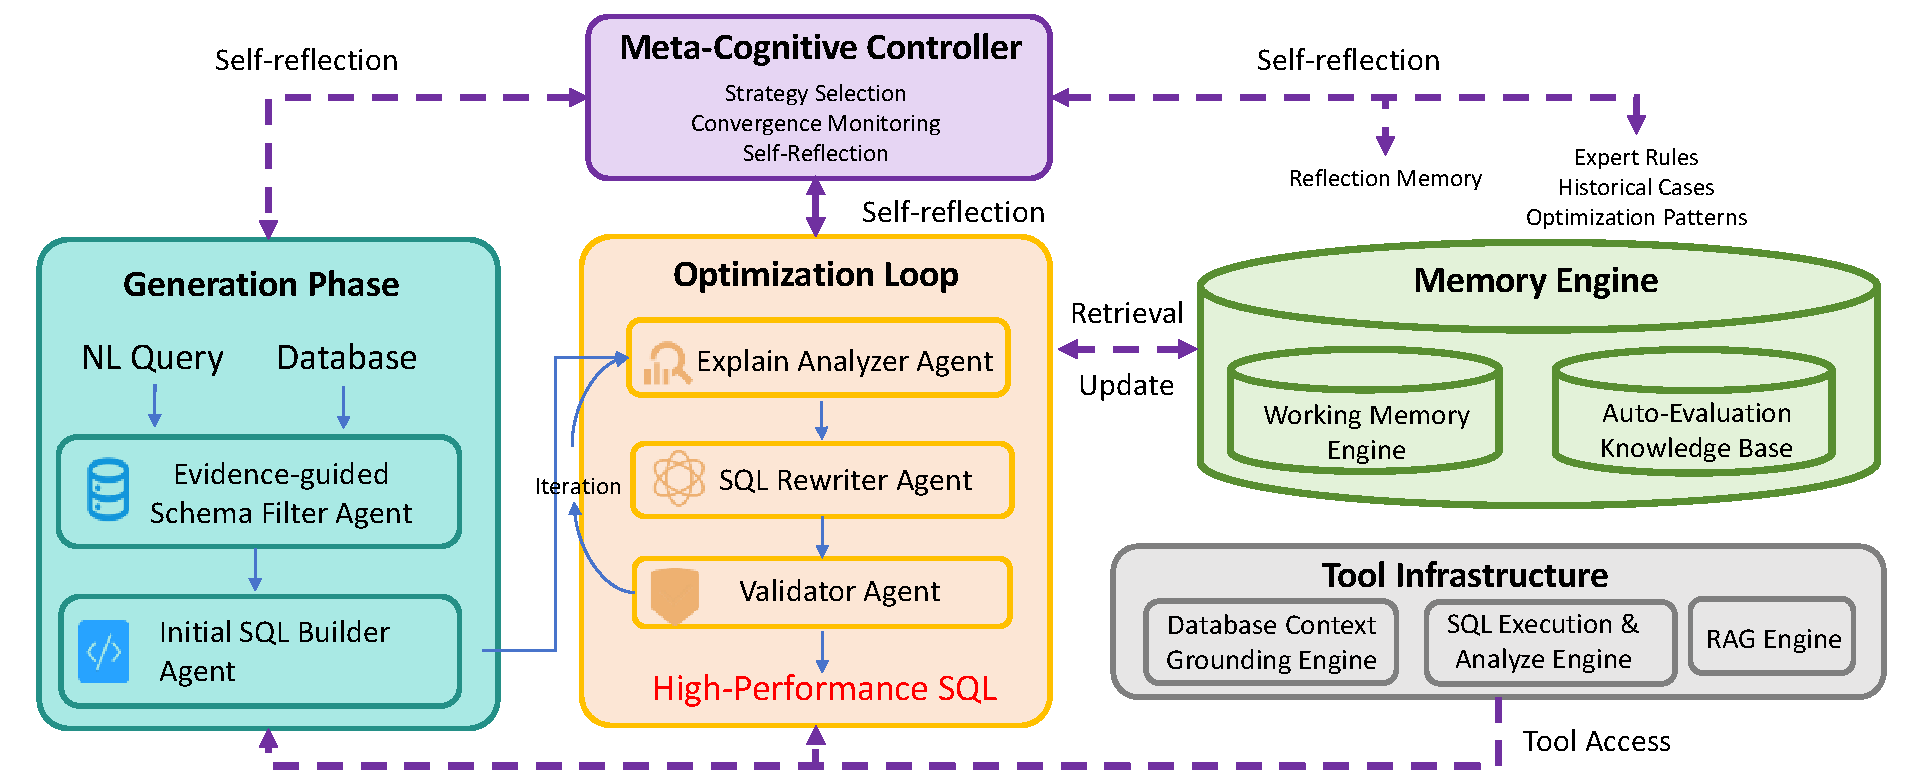
\includegraphics[width=0.92\linewidth]{./images/overview.pdf} 
	\vspace{-3mm}
	\caption{\textbf{Overview of \toolname}}
	\label{fig:overview}
	\vspace{-6mm}
\end{figure*}

The remainder of this section describes each component of \toolname.
We first present the Generation Phase for constructing an initial SQL query (Section~\ref{subsec: Generation Phase}), followed by the Optimization Loop for execution- and plan-aware rewriting (Section~\ref{subsec: Optimization Loop}).
We then introduce the Meta-Cognitive Controller that orchestrates these processes through strategy selection, monitoring, and self-reflection (Section~\ref{subsec: Meta-Cognitive Controller}).
Finally, we describe the Memory Engine and Tool Infrastructure that support retrieval, experience accumulation, and database feedback (Section~\ref{subsec: Memory Engine and Tool Infrastructure}).
Due to space limitations, we also release a detailed case study in our GitHub repository~\cite{optsql_case_study} to illustrate how \toolname\ realizes its key designs.

\subsection{Generation Phase}
\label{subsec: Generation Phase}
The Generation Phase aims to construct a set of executable and semantically plausible initial SQL candidates based on the question and database environment.
It focuses on two core capabilities: evidence construction and multi-strategy SQL generation.

\textbf{Evidence-guided Schema Filter Agent.}
This agent is responsible for grounding the input question into a compact, relevant, and executable schema context for downstream SQL generation.
It combines robust schema linking with value grounding, aiming to identify not only the tables and columns mentioned or implied by the question, but also the concrete database values and conditions needed to express the user intent.
To improve schema robustness, the agent supports multiple complementary schema linking strategies:

\begin{itemize}[leftmargin=10pt]
	\item \textit{Direct schema linking} maps the natural language question to relevant tables and columns by reasoning over question semantics and schema descriptions.
	This strategy is effective when the question contains explicit lexical or semantic cues.
	
	\item \textit{Reverse schema linking} hypothesizes a tentative SQL structure and then extracts the tables and columns implied by this structure~\cite{li2026deepeye}.
	This recovers latent schema dependencies, such as join tables, grouping columns, or aggregation-related attributes, that may be missed by direct matching.
	
	\item \textit{Value-grounded schema linking} identifies relevant schema elements through actual database contents.
	Instead of relying only on table or column names, the agent checks whether values in a column match or semantically correspond to phrases in the question, which is especially useful when schema names are ambiguous or weakly informative.
\end{itemize}

Beyond schema linking, the agent further performs active value grounding to translate natural language expressions into concrete database predicates.
It supports several value grounding capabilities:

\begin{itemize}[leftmargin=10pt]
	\item \textit{Exact value verification} checks whether a phrase in the question directly appears in candidate columns.
	This is useful for grounding categorical conditions such as names, locations, statuses, or labels.
	
	\item \textit{Semantic value matching} retrieves column values that are semantically close to question phrases, allowing the agent to handle paraphrases, abbreviations, and domain-specific expressions.
	
	\item \textit{Distinct-value inspection} examines representative or unique values of a column to infer how natural language concepts are encoded in the database, such as whether a Boolean concept is represented by \texttt{0}/\texttt{1}, \texttt{Y}/\texttt{N}, or textual labels.
	
	\item \textit{Data sampling and distribution checking} inspects example rows or value distributions to understand column semantics and avoid grounding predicates on irrelevant or sparsely populated columns.
	
	\item \textit{Null and type analysis} checks whether candidate columns contain nulls or unexpected value formats, helping the agent avoid unreliable predicates and distinguish categorical, numerical, date, and Boolean constraints.
	
	\item \textit{Composite predicate grounding} combines multiple grounded values or columns when a natural language phrase corresponds to a compound condition, such as a grade span, date range, or multi-attribute status.
\end{itemize}

For example, a phrase such as ``kindergarten to 8th grade'' may be grounded as \texttt{Low\_Grade = 'K'} and \texttt{High\_Grade = '8'}, while ``magnet program'' may correspond to a binary or categorical value after inspecting the value distribution of a related column.
These grounded facts are passed to the SQL generator as explicit evidence, reducing the risk of hallucinated predicates or incorrect value choices.
Finally, the agent further completes the relational context required for SQL construction.
The selected schema elements may be semantically relevant but structurally disconnected; for example, two relevant tables may require intermediate tables or primary--foreign key columns to form a valid join path.
Therefore, the agent supplements necessary join keys and bridge tables according to the database relationships, so that the resulting schema context can support executable SQL generation.
The output of this agent is an evidence-enriched schema context that integrates schema relevance, verified value grounding, ambiguous-case evidence, and join-path information for downstream SQL generation.

\textbf{Initial SQL Builder Agent.}
Initial SQL Builder Agent is responsible for producing executable and semantically plausible initial SQL candidates.
It provides a set of complementary SQL construction capabilities, rather than a fixed generation pipeline.
Depending on the task complexity, schema ambiguity, and control signals from the Meta-Cognitive Controller, the agent may invoke one or more generation strategies to balance robustness and efficiency.
The agent supports the following SQL generation strategies:

\begin{itemize}[leftmargin=10pt]
	\item \textit{Skeleton-based generation} follows a top-down construction process.
	It first analyzes the required SQL components, such as selection, filtering, joining, grouping, and ordering, then sketches a SQL skeleton, and finally fills in concrete tables, columns, predicates, and functions.
	This strategy is useful for queries that require clear structural planning.
	
	\item \textit{ICL-based generation} leverages retrieved demonstrations to guide SQL construction.
	By retrieving structurally similar examples, the agent can reuse successful query patterns and adapt them to the current grounded schema.
	This strategy is especially helpful when the question resembles previously observed SQL structures.
	
	\item \textit{Decomposition-based generation} breaks a complex question into simpler sub-questions and generates SQL fragments for each sub-task before composing them into a complete query.
	This strategy is designed for complex analytical questions involving nested reasoning, multiple conditions, or multi-step aggregation.
\end{itemize}

After candidate generation, the agent can apply a lightweight repair loop to improve executability.
It checks basic syntactic and execution errors, and revises invalid candidates using the original question, grounded schema evidence, and database error messages.
This repair process removes obvious generation failures before candidate selection, while leaving global strategy switching and deeper optimization to the Meta-Cognitive Controller.
When the controller activates multiple generation strategies, the agent may produce multiple candidate SQLs.
In this case, the agent further performs \textit{execution-based selection}.
Candidates are grouped according to their execution results, and each group is treated as a behavioral cluster.
If one cluster forms a dominant majority, the agent selects a representative query from that cluster as the initial SQL.
Otherwise, representative candidates from the top clusters are compared through pairwise semantic judgment, and each candidate is ranked by a confidence-aware score.
The candidate with the highest score is selected as the output of the Initial SQL Builder Agent.


\subsection{Optimization Loop}
\label{subsec: Optimization Loop}

The Optimization Loop aims to improve the execution efficiency of an initial SQL query while preserving its semantics.
It is activated by the Meta-Cognitive Controller when the generated SQL may benefit from further optimization.
The loop consists of three agents: the Explain Analyzer Agent, the SQL Rewriter Agent, and the Validator Agent.

\textbf{Explain Analyzer Agent.}
This agent is responsible for diagnosing potential inefficiencies in the current SQL query and producing optimization suggestions for the SQL Rewriter Agent.
Given an initial SQL query, it first obtains the query plan from the database and normalizes raw plan operators into stable bottleneck signals.
These plan-level signals are then combined with lightweight SQL-structure analysis and schema statistics, such as table size, available indexes, and nullable columns, to decide whether the observed behavior is likely to be a real bottleneck.
The agent then maps each bottleneck signal to one or more candidate rewrite directions.
For instance, consider a query such as ``\texttt{SELECT order\_id, customer\_id, order\_date FROM orders WHERE status = 'shipped' ORDER BY order\_date LIMIT 10}''.
If the query plan contains both \texttt{SCAN orders} and \texttt{USE TEMP B-TREE FOR ORDER BY}, the agent derives two signals: \texttt{full\_table\_scan} and \texttt{temp\_sort}.
When \texttt{orders} is a large table, the full scan indicates a potentially expensive access path and may trigger access-path-aware suggestions, while the temporary sort may suggest aligning the \texttt{ORDER BY}/\texttt{LIMIT} pattern with available ordering or indexes.
The output of the agent is therefore a set of suggestions, such as \textit{missing filter pushdown} or \textit{inefficient ordering}, rather than a rewritten SQL query.

As shown in Table~\ref{tab:explain-analyzer}, the agent maintains a set of optimization patterns.
Each pattern describes a possible inefficiency, a candidate rewrite direction, and an applicability condition that constrains when the rewrite can be attempted without changing query semantics.
These suggestions are not directly applied as deterministic rules.
Instead, they serve as evidence for the SQL Rewriter Agent, which decides how to rewrite the query under semantic-preservation constraints.


%Table I 具体解释：
%Redundant projection：主要处理 SELECT * 或输出不必要列的问题。它可以减少数据传输、物化和排序/聚合时的中间结果宽度。但只有当所需输出列能从 NL question 或 SQL 语义中确定时才能改。
%Scalar MAX/MIN subquery：例如把某些 MAX(x) / MIN(x) 查询改成 ORDER BY x DESC/ASC LIMIT 1。这种 rewrite 在有索引时可能更快，但要注意 NULL、tie 和返回列语义。
%Correlated subquery：把逐行执行的相关子查询改成 JOIN 或 CTE，可能减少重复计算。但要特别注意 duplicate、NULL、EXISTS/IN、聚合和 cardinality 变化。
%Missing filter pushdown：把选择性过滤条件尽量提前到 base table 或 CTE 内部，减少后续 join/aggregation 的输入规模。但不能跨越会改变语义的 outer join、aggregation、window function 或 volatile expression。
%Late aggregation：在 join 之前先聚合，减少 join 输入规模。这个很有用，但必须保证 grouping key、join multiplicity 和 aggregate semantics 不变。
%Inefficient OR predicate：将复杂 OR 谓词改成 UNION / UNION ALL。这个可能让每个分支利用索引，但要处理重复行和 predicate overlap。
%Redundant join path：删除不必要的 join 或 bridge table。但要保证这个 join 没有隐式过滤、去重或改变行数。
%Function on indexed column：例如把 DATE(timestamp_col) = '2024-01-01' 改成 range predicate，使索引可用。要保证函数等价转换成立。
%Inefficient ordering：处理不必要排序、排序表达式阻碍索引、ORDER BY 与 LIMIT 搭配低效等问题。

\begin{table*}[t]
	\centering
	\vspace{-3mm}
	\caption{\textbf{Representative optimization patterns used by the Explain Analyzer Agent.}}
	\vspace{-2mm}
	\label{tab:explain-analyzer}
%	\small
%	\scriptsize
	\fontsize{6.4pt}{6.8pt}\selectfont
	\renewcommand{\arraystretch}{0.92}
	\begin{tabular}{p{0.14\linewidth}p{0.31\linewidth}p{0.45\linewidth}}
		\toprule
		\textbf{Pattern} & \textbf{Rewrite Direction} & \textbf{Applicability Condition} \\
		\midrule
		Redundant projection
		& Replace \texttt{SELECT *} with necessary projected columns.
		& Applied when required output columns can be inferred from the question or generated SQL. \\
		
		Scalar \texttt{MAX}/\texttt{MIN} subquery
		& Rewrite to \texttt{ORDER BY ... LIMIT 1}.
		& Applied only when tie behavior and aggregation semantics are preserved. \\
		
		Correlated subquery
		& Rewrite to \texttt{JOIN} or \texttt{CTE}.
		& Applied when an equivalent rewrite pattern is retrieved or can be validated. \\
		
		Missing filter pushdown
		& Move selective predicates closer to base tables.
		& Applied when predicate movement does not change join or aggregation semantics. \\
		
		Late aggregation
		& Pre-aggregate before join.
		& Applied when grouping keys and aggregation semantics remain equivalent. \\
		
		Inefficient \texttt{OR} predicate
		& Rewrite to \texttt{UNION} or \texttt{UNION ALL}.
		& Applied when duplicate semantics are correctly handled. \\
		
		Redundant join path
		& Simplify unnecessary joins or bridge tables.
		& Applied only when projected columns and filtering semantics are unaffected. \\
		
		Function on indexed column
		& Rewrite to an equivalent range or comparison predicate.
		& Applied when the transformation preserves value semantics. \\
		
		Inefficient ordering
		& Align \texttt{ORDER BY} / \texttt{LIMIT} with available ordering or indexes.
		& Applied when ordering semantics are unchanged. \\
		\bottomrule
	\end{tabular}
	\vspace{-5mm}
\end{table*}

\textbf{SQL Rewriter Agent.}
The SQL Rewriter Agent transforms the current SQL query into a potentially more efficient variant based on the suggestions produced by the Explain Analyzer Agent.
Its input includes the original SQL, the detected bottleneck signals, the corresponding rewrite directions, the applicability conditions, and optionally retrieved rewrite cases from the Memory Engine.
The rewriter does not freely optimize the query; instead, it is constrained to apply rewrite actions that are supported by the available evidence.
%For low-risk cases, such as redundant projection, the rewriter may directly replace \texttt{SELECT *} with the columns required by the question or the current SQL.
%For more semantics-sensitive cases, such as correlated-subquery rewriting, pre-aggregation before joins, or rewriting \texttt{OR} predicates to \texttt{UNION}, the rewriter relies on retrieved templates, explicit applicability conditions, or strong structural evidence before attempting the transformation.
%For example, if the Explain Analyzer reports an \textit{inefficient ordering} pattern, the rewriter may restructure the query to better align the \texttt{ORDER BY}/\texttt{LIMIT} clause with available ordering or access paths, but only when the ordering semantics remain unchanged.
%The output of this agent is a rewritten SQL query together with a brief rationale describing which suggestion is applied and why the rewrite is expected to reduce cost.

\textbf{Validator Agent.}
The Validator Agent determines whether a rewritten SQL query should be accepted.
It performs two checks.
First, it checks semantic consistency between the original SQL and the rewritten SQL, ensuring that the rewrite does not change the intended query result.
Second, it evaluates whether the rewritten SQL improves execution efficiency using available database feedback including estimated optimizer cost and execution latency.
%
If the rewritten SQL fails the semantic-consistency check, it is rejected and returned to the Meta-Cognitive Controller for reflection.
The controller may then ask the SQL Rewriter Agent to retry with the original SQL, the failed rewrite, and the validation feedback.
If the rewritten SQL preserves semantics but does not reduce cost, the controller may retry with another rewrite direction, retrieve additional cases from the Memory Engine, or terminate the optimization loop when further improvement is unlikely.
Only rewrites that pass both semantic consistency and cost-improvement checks are accepted as optimized outputs.

\vspace{-2mm}
\subsection{Meta-Cognitive Controller}
\label{subsec: Meta-Cognitive Controller}
The Meta-Cognitive Controller is the central coordination module of OPTSQL. It maintains a global task state, selects which agent capabilities should be invoked, monitors intermediate feedback, and decides whether the system should continue, switch strategy, or terminate.
\revision{Algorithm~\ref{alg:meta-controller} formalizes the Meta-Cognitive Controller as a state-based control loop shared by generation and optimization.
The workflow defines the available agent capabilities and their execution rules; within this workflow, the LLM interprets feedback and chooses what to do next.
We follow the algorithm below from state initialization through action selection to validation and termination.}

\begin{algorithm}[t]
\renewcommand{\revision}[1]{#1}
\color{black}
\small
\caption{\revision{Meta-cognitive control of generation and optional optimization}}
\label{alg:meta-controller}
\begin{algorithmic}[1]
\algrenewcommand{\algorithmiccomment}[1]{\hfill\textcolor{blue}{//~#1}}
\Require \revision{Question $x$, database $\mathcal{D}$, AEKB $K$}
\Ensure \revision{Selected SQL $q$, or $\bot$ if generation fails}
\Statex \revision{\textcolor{blue}{// Initialize the State}}
\State \revision{Initialize working-memory state $s$ from $(x,\mathcal{D})$; $q\gets\bot$}\label{algmc:init}
\Statex \revision{\textcolor{blue}{// Set Up the Current Phase}}
\For{\revision{$p\in[\text{generation},\text{optimization}]$}}\label{algmc:phase}
    \State \revision{If $p=\text{optimization}$ and $\operatorname{Optimize}_{\mathrm{LLM}}(s)=\mathrm{false}$, \textbf{return} $q$}\label{algmc:gate}
    \State \revision{$U\gets\operatorname{Catalog}(p)$}\label{algmc:catalog}\Comment{\revision{$U$: remaining action identifiers}}
    \Statex \revision{\textcolor{blue}{// Observe Signals and Identify Eligible Actions}}
    \While{\revision{$U\ne\varnothing$}}\label{algmc:loop}
        \State \revision{$\sigma\gets\operatorname{Signals}(s)$}\label{algmc:signals}\Comment{\revision{$\sigma$: Boolean flags for grounding, candidate, plan, and rewrite issues}}
        \State \revision{$A\gets\operatorname{Eligible}(U,s)\cup\operatorname{AllowedStop}(p,s)$}\label{algmc:eligible}\Comment{\revision{$A$: eligible actions, including a permitted stop}}
        \If{\revision{$A=\varnothing$}}\label{algmc:empty}
            \State \revision{\textbf{break}}\label{algmc:emptybreak}
        \EndIf
        \Statex \revision{\textcolor{blue}{// Reflect, Select, and Adapt}}
        \State \revision{$r\gets\operatorname{Reflect}_{\mathrm{LLM}}(s,\sigma)$ if $\operatorname{NeedsReflection}(\sigma)$, else $\varnothing$}\label{algmc:reflect}\Comment{\revision{$r$: issue, supporting evidence, and next-step constraint}}
        \State \revision{$\tilde a\gets\operatorname{Propose}_{\mathrm{LLM}}(s,\sigma,r,A)$}\label{algmc:propose}\Comment{\revision{$\tilde a$: proposed action identifier and arguments}}
        \State \revision{$a\gets\operatorname{CheckOrFallback}(\tilde a,A,s,p)$}\label{algmc:guard}\Comment{\revision{$a$: checked proposal or valid fallback}}
        \If{\revision{$a=\textsc{Stop}$}}\label{algmc:stop}
            \State \revision{\textbf{break}}\label{algmc:stopbreak}
        \EndIf
        \State \revision{$U\gets U\setminus\{\operatorname{id}(a)\}$; $o\gets\operatorname{Execute}(a,s,K)$}\label{algmc:execute}\Comment{\revision{$o$: agent report containing outputs, feedback, or errors}}
        \Statex \revision{\textcolor{blue}{// Validate the Output and Update the State}}
        \If{\revision{$a$ is a rewrite action and $o.\mathrm{sql}\ne\bot$}}
            \State \revision{$q'\gets o.\mathrm{sql}$}\label{algmc:extract}
            \State \revision{$v\gets\operatorname{Validate}(q,q',\mathcal{D})$}\label{algmc:validate}\Comment{\revision{$v$: execution, consistency, and cost-check results}}
            \If{\revision{$v.\mathrm{success}\land v.\mathrm{consistent}\land v.\mathrm{costImproved}$}}\label{algmc:accept}
                \State \revision{$K\gets\operatorname{StoreValidatedCase}(K,q,q',v)$}\label{algmc:store}
                \State \revision{$q\gets q'$; $o.P\gets\operatorname{Analyze}(q,\mathcal{D})$}\label{algmc:refresh}
            \EndIf
            \State \revision{$o.v\gets v$; attach the acceptance decision to $o$}\label{algmc:feedback}
        \EndIf
        \State \revision{$s\gets\operatorname{Update}(s,a,\sigma,r,o)$}\label{algmc:update}
    \EndWhile
    \Statex \revision{\textcolor{blue}{// Complete the Phase and Return the Query}}
    \If{\revision{$p=\text{generation}$}}
        \State \revision{$q\gets\operatorname{BuilderSelect}(s.Q)$}\label{algmc:select}
        \If{\revision{$q=\bot$}}
            \State \revision{\textbf{return} $\bot$}
        \EndIf
    \EndIf
\EndFor
\State \revision{\textbf{return} $q$}\label{algmc:return}
\end{algorithmic}
\end{algorithm}

\revision{\textbf{Initialize the State (line~\ref{algmc:init}).}
For a question $x$ and database $\mathcal{D}$, the Memory Engine initializes the task's working memory, whose structured state is
\[
 s=\langle E,Q,q,P,V,H\rangle.
\]
The controller reads and updates this same state. All symbols refer to the current iteration and are updated in place, as in Algorithm~\ref{alg:meta-controller}.
Here, $E$ contains the question and database context, task-complexity observations, and grounding evidence, including schema/value alternatives, join paths, and evidence reliability.
$Q$ stores generated candidates with their strategies, execution and local-repair outcomes, result clusters, and confidence scores; $q$ identifies the currently selected query.
$P$ contains the current query's plan, cost observations, bottlenecks, applicable rewrite directions, and retrieved AEKB cases.
$V$ stores validation reports linked to each source--rewrite pair, including consistency results, cost changes, and acceptance decisions.
$H$ is the action history, recording strategies, arguments, reflection records, outputs, and feedback, including unsuccessful attempts.
Initially, $E$ contains the input question and available database context, $q=\bot$, and the remaining fields are empty.
Throughout the algorithm, $q$ denotes the query component of $s$, so assigning $q$ directly updates that component; AEKB $K$ remains separate from the task-local state.}

\revision{\textbf{Set Up the Current Phase (lines~\ref{algmc:phase}--\ref{algmc:catalog}).}
The controller first enters generation and then, if needed, optimization.
The optimization decision (line~\ref{algmc:gate}) is evaluated only after generation has selected an initial SQL; the LLM uses that query, database context, and accumulated feedback to decide whether to continue.
For each phase, $U$ contains its available action identifiers: evidence gathering and SQL construction during generation, or plan analysis, case retrieval, and direction-specific rewriting during optimization.
An identifier specifies a capability and strategy, with separate identifiers for an initial attempt and its feedback-guided revision; the arguments are supplied from the current state.
This finite catalog encodes the capabilities described in Sections~\ref{subsec: Generation Phase} and~\ref{subsec: Optimization Loop}, while leaving their selection and order to the controller.}

\revision{\textbf{Observe Signals and Identify Eligible Actions (lines~\ref{algmc:loop}--\ref{algmc:emptybreak}).}
At each iteration, $\sigma=\operatorname{Signals}(s)$ summarizes four Boolean indicators $(g,e,b,f)$: unresolved grounding or missing join paths ($g$), unresolved candidate execution errors or result disagreement ($e$), supported current-plan bottlenecks ($b$), and a failed or non-improving rewrite of the current source query ($f$) (line~\ref{algmc:signals}).
These indicators describe the current unresolved issues, rather than every past failure in the history; supporting details remain in $s$.
The program then forms $A$ by filtering the remaining actions in $U$ against their preconditions (line~\ref{algmc:eligible}).
SQL construction requires schema context; rewriting requires an executable selected query and an applicable direction; a revision requires feedback from its initial attempt, referring to the still-current source SQL for rewrite retries.
The program also permits stopping generation once an executable candidate exists, and permits stopping optimization while retaining the current query.
If $A$ is empty, the phase ends.}

\revision{\textbf{Reflect, Select, and Adapt (lines~\ref{algmc:reflect}--\ref{algmc:execute}).}
The program explicitly sets $\operatorname{NeedsReflection}(\sigma)=g\lor e\lor f$; when true, the LLM produces the following reflection record (line~\ref{algmc:reflect}):
\[
 r=\langle\text{issue},\text{supporting feedback},\text{next-step constraint}\rangle;
\]
otherwise, $r$ is empty; a malformed reflection record is also treated as empty.
For example, a failed consistency check identifies which query behavior changed and supplies a semantic constraint for the next rewrite.
Given $(s,\sigma,r,A)$, the LLM proposes an action identifier and its arguments (line~\ref{algmc:propose}); it can gather more evidence, switch SQL construction strategies, retrieve cases, retry a rewrite with feedback, choose another direction, or stop, subject to the current phase.
Thus, $\sigma$ controls whether reflection occurs and directly informs action selection even when $r$ is empty.
This state-dependent choice implements adaptation: the next capability and its inputs depend on the current evidence and reflection, rather than a fixed sequence of agent calls.
The program checks the proposal against $A$ and available state objects; an invalid proposal falls back to the first eligible non-stop action in catalog order with state-bound arguments, or to an allowed stop if none remains (line~\ref{algmc:guard}).
For a non-stop action, the program consumes its identifier and invokes the selected agent (line~\ref{algmc:execute}); SQL-building actions include the Builder's local execution-error repair, while process-level strategy switching remains with the controller.
$\operatorname{Execute}$ returns a structured report $o$ rather than directly replacing $q$; every report has $o.\mathrm{sql}=\bot$ unless it contains a proposed rewrite, and failures are returned as error reports for the common state-update step.}

\revision{\textbf{Validate the Output and Update the State (lines~\ref{algmc:extract}--\ref{algmc:update}).}
A proposed rewrite is explicitly extracted as $q'=o.\mathrm{sql}$ (line~\ref{algmc:extract}) before validation against the current query.
The Validator returns Boolean fields $v.\mathrm{success}$, $v.\mathrm{consistent}$, and $v.\mathrm{costImproved}$: successful execution, matching results on the available database state, and $C(q')<C(q)$ for $C(q)=\mathrm{Cost}(q,\mathcal{D})$ under the same measure and environment (lines~\ref{algmc:validate}--\ref{algmc:accept}).
Each field is false unless its check succeeds; missing or incomparable costs make $v.\mathrm{costImproved}$ false, so a failed check cannot accept a rewrite.
On acceptance, the Memory Engine stores the validated case in AEKB, $q'$ replaces $q$, and plan feedback is refreshed (lines~\ref{algmc:store}--\ref{algmc:refresh}); on rejection, $q$ remains unchanged and the failure stays in working memory (line~\ref{algmc:feedback}).
After every action, $\operatorname{Update}$ merges the agent report into the appropriate fields of $s$ and appends $(a,\sigma,r,o,q)$ to $H$, completing the cycle back to observation (line~\ref{algmc:update}).
This merge preserves the selected-query field: $q$ is assigned only by candidate selection or an accepted rewrite, so a failed action cannot overwrite it.
Evidence-gathering outputs update $E$, generation outputs update $Q$, plan analysis and retrieval update $P$, and rewrite checks update $V$; the reflection record $r$ is retained in $H$.
When $q$ changes, plan information is refreshed and retrieved-case applicability is rechecked for the new query; earlier observations remain accessible through $H$. If plan analysis fails, the old plan is invalidated and the error is recorded; only newly supported directions are eligible for rewriting.
%Neither selection nor validation uses benchmark reference SQL, and consistency on the available database state does not establish equivalence on every possible database instance.
}

\revision{\textbf{Complete the Phase and Return the Query (lines~\ref{algmc:select}--\ref{algmc:return}).}
When generation ends, the SQL Builder selects an executable initial query, or returns $\bot$ if none exists.
The controller optionally optimizes this query and returns the latest accepted result.
Each phase ends on a permitted stop or when no eligible action remains; executed action identifiers are removed from the finite set $U$.
The LLM supplies reflection and adaptive selection, while workflow and validation rules are manually specified; AEKB updates store validated cases without changing model parameters.}

\subsection{Memory Engine and Tool Infrastructure}
\label{subsec: Memory Engine and Tool Infrastructure}
\textbf{Memory Engine.}
\revision{The Memory Engine manages two stores: task-local working memory and the reusable AEKB $K$.
Working memory holds exactly the controller state $s=\langle E,Q,q,P,V,H\rangle$ defined in Section~\ref{subsec: Meta-Cognitive Controller}.
Its fields provide the controller's current view of task context and grounding ($E$), generated candidates ($Q$), the selected query ($q$), plan and retrieval context ($P$), validation outcomes ($V$), and the action trace ($H$).
The controller supplies decisions and agent reports; the Memory Engine records them in these fields through the update step of Algorithm~\ref{alg:meta-controller}.
Thus, working state and working memory refer to the same task-local information, with $H$ preserving the history behind the current state.
%Working memory is initialized afresh for each input question and retained throughout that question's generation and optimization phases.
}

\revision{The AEKB contains static expert rules and reusable rewrite cases, rather than the full task state or action trace.
Retrieval places relevant cases in $P$ for the current query without changing the AEKB.
A new case is added to $K$ only when a rewrite executes successfully, preserves the source query's observed results, and reduces cost under the same measure and environment.
Failed rewrites and their diagnoses remain in $V$ and $H$ and are not promoted to reusable knowledge.
The accepted case is summarized into the template record below; this promotion does not copy the question's entire working memory into $K$.
%Unlike task-local working memory, $K$ can carry accepted cases across questions within a run; its reset between repeated evaluation runs follows Section~\ref{sec:evaluation}.
}
% Previous memory description retained for comparison.
% The Memory Engine supports both task-level reasoning and cross-task experience reuse.
% It consists of working memory and the AEKB.
% %The working memory stores the intermediate trace of the current task.
% %It records the database environment, question complexity, selected strategies, schema and value evidence, generated SQL candidates, execution errors, repair attempts, optimization hints, retrieved cases, rewritten SQLs, validation results, and cost changes.  \lin{Recheck}
% The working memory stores the structured task state and intermediate trace of the current task.
% It records task context, including the database environment, question complexity, and available statistics or indexes.
% It also stores grounding evidence, including selected tables and columns, grounded values, ambiguous schema or value alternatives, join-path evidence, and evidence reliability.
% During SQL generation, it records selected generation strategies, generated SQL candidates, execution errors, repair attempts, execution-result clusters, candidate confidence, and the selected initial SQL.
% During optimization, it records query plans, normalized bottleneck signals, optimization hints, rewrite directions, applicability conditions, retrieved cases, rewritten SQLs, semantic validation results, estimated costs, execution latency, and cost changes.
% The Meta-Cognitive Controller uses this memory to avoid repeated failed actions and provide context for subsequent reflection, retry, and termination decisions.
% Failed rewrites are kept only in working memory as task-level negative feedback, rather than being promoted to reusable knowledge.
% %
% The AEKB stores reusable optimization knowledge.
% It contains expert rules and historical rewrite cases validated by the Validator Agent.
% A rewrite is added to the AEKB only when it satisfies two conditions: the rewritten SQL is semantically consistent with the original SQL, and it reduces execution cost.
% 
Each accepted case is summarized as a rewrite template record:
\[
\langle T_{\mathit{src}}, T_{\mathit{dst}}, C, R \rangle .
\]
Here, ($T_{\mathit{src}}$) denotes the source SQL template, ($T_{\mathit{dst}}$) denotes the rewritten SQL template, ($C$) specifies the applicability constraints, and ($R$) describes the optimization rationale.
%
To retrieve relevant cases, the RAG Engine first normalizes the current SQL into a template.
It parses the SQL into an AST, replaces table names with \texttt{TABLE}, replaces column names with coarse semantic tokens such as \texttt{TEXT\_COLUMN}, \texttt{NUMERIC\_COLUMN}, \texttt{DATE\_COLUMN}, \texttt{ID\_COLUMN}, and \texttt{FK\_COLUMN}, replaces literals with \texttt{LITERAL}, and normalizes whitespace and case.
The normalized template is then compared with the ($T_{\mathit{src}}$) templates in the AEKB using a hybrid similarity score that combines sequence similarity and token-set overlap.
The top-ranked records are returned as candidate rewrite knowledge for the SQL Rewriter Agent.
Through this mechanism, \toolname\ accumulates validated optimization experience and reuses it to guide future bottleneck analysis and rewrite selection.



\textbf{Tool Infrastructure.}
The Tool Infrastructure provides executable interfaces between the agents and the database environment.
It consists of three groups of tools:

\begin{itemize}[leftmargin=10pt]
	\item \textit{Database Context Grounding Engine.}
	This engine supports schema and value evidence construction for the Evidence-guided Schema Filter Agent.
	It provides operations for schema linking, value verification, semantic value matching, distinct-value inspection, data sampling, null/type analysis, and relational completion.
	These tools help the system ground NL expressions into relevant tables, columns, values, and join paths.
	
	\item \textit{SQL Execution and Analysis Engine.}
	This engine supports execution-aware optimization for the Optimization Loop.
	It includes a query plan analyzer, a SQL quality analyzer, a semantic consistency checker, and a cost evaluator.
	The query plan analyzer normalizes raw query plans into plan-level risk signals, while the SQL quality analyzer detects static SQL risks from the parsed AST.
	The semantic consistency checker compares the original and rewritten SQLs on the available database state, and the cost evaluator measures estimated optimizer cost and execution latency before and after rewriting.
	
	\item \textit{RAG Engine.}
	This engine supports memory retrieval and update.
	It provides a SQL formatter for template normalization, a retriever for selecting relevant rewrite cases, and an updater for inserting validated optimization cases into the AEKB.
	These tools allow the SQL Rewriter Agent to reuse prior optimization experience and update the knowledge base after successful rewrites.
\end{itemize}

Together, these tools allow \toolname\ to ground reasoning in database evidence, analyze execution behavior, retrieve relevant optimization experience, and update memory after successful rewrites.


%\section{Case Study}
%\label{sec:case study}

\endgroup
	%\vspace{-3mm}
\section{Experiment}
\label{sec:evaluation}

% 减少公式之间的间距
\begingroup
\setlength{\abovedisplayskip}{3pt}
\setlength{\belowdisplayskip}{3pt}
\setlength{\abovedisplayshortskip}{2pt}
\setlength{\belowdisplayshortskip}{2pt}
\setlength{\jot}{2pt}

% EX VES CR AR@1 AR@0.8
% Baselines:
% -  开源基础模型 + 闭源基础模型： GPT-5.4、Deepseek、Qwen-7B、XiYanSQL-7B、Llama-8B (选3-4个模型)
% -  Text-to-SQL Agentic / Approach : 
		%Multi-Agent Approach： Agentar-Scale-SQL、MAC-SQL、CHESS
%		%Single-Agent Appraoch:  DIN-SQL、DAIL-SQL
% Benchmark: BIRD and EESQLBench

% RQ1： Overall Performance  表格可以参考 LEAF-SQL: Level-wise Exploration with Adaptive Fine-graining for Text-to-SQL Skeleton Prediction、SchemaRAG
% RQ2： Ablation Study
% RQ3:  Case Study


%- BaseLines
%1. （2种）基于 Prompt 的方法：DIN-SQL，DAIL-SQL
%2. （3种）基于 Agent 的方法：
%- MAC-SQL，DeepEye
%- CHESS（需要再看一下结果）
%3. （2种）基于微调模型的方法（基于原始 BIRD pipeline）：XiYan-SQL（QwenCoder-32B-2504） + OmniSQL(32B)
%
%- LLMs
%- Qwen3-Coder-30B-A3B-Instruct
%- CodeLlama-34b-Instruct-hf
%- DeepSeek-v4-pro
%- GPT-5.4


% Performance Evaluation  (Token 消耗)
% Ablation Study
% Error Analysis

% 统计显著性检验
% 重复运行5次?


%\vspace{-2mm}
\subsection{Experimental Setup}
\textbf{Datasets.}
We evaluate \toolname\ on two complementary benchmarks: \textbf{\textsc{BIRD}}~\cite{li2023can} and \textbf{\textsc{EESQLBench}}~\cite{lin2026cracking}.
%\begin{itemize}[leftmargin=10pt]
\textsc{BIRD} is a widely used cross-domain Text-to-SQL benchmark, containing more than 12,751 question--SQL pairs over 95 large-scale databases and 37 professional domains.
It features realistic database scenarios with complex schemas, domain-specific knowledge, and noisy data, making it suitable for evaluating the general Text-to-SQL capability of \toolname.
%
To further evaluate the generality and efficiency-oriented capability of \toolname, we use \textsc{EESQLBench}, an efficiency-focused benchmark where each NL question is paired with an expert-optimized canonical SQL query.
% containing 213 tasks,
Its tasks include large databases, complex joins, nested subqueries, and optimization-sensitive predicates, enabling us to assess whether \toolname\ can generate SQL queries that are not only semantically correct but also close to human expert-level efficiency.
%\end{itemize}

\textbf{Metrics.}
We evaluate both semantic correctness and execution efficiency.
Let $q_i^*$ be the canonical SQL, $\hat{q}_i$ be the generated SQL, $S_i$ be the database, and $N$ be the number of test instances.
We define:
\[
\mathbf{1}_i =
\begin{cases}
	1, & \mathrm{Exec}(\hat{q}_i,S_i)=\mathrm{Exec}(q_i^*,S_i),\\
	0, & \text{otherwise}.
\end{cases}
\]

\textbf{\textit{Execution Accuracy (EX)}}~\cite{li2023can} measures the fraction of semantically correct outputs:
\[
\mathrm{EX}=\frac{1}{N}\sum_{i=1}^{N}\mathbf{1}_i.
\]
It evaluates whether the generated SQL produces the correct result, regardless of efficiency.

\textbf{\textit{Valid Efficiency Score (VES)}}~\cite{li2023can} measures runtime-based efficiency for valid outputs:
\[
\mathrm{VES}=
\frac{1}{N}\sum_{i=1}^{N}
\mathbf{1}_i
\cdot
\sqrt{\frac{T(q_i^*,S_i)}{T(\hat{q}_i,S_i)}} ,
\]
where $T(q,S)$ denotes execution time.
VES rewards generated SQLs that are both correct and fast, but it may be affected by runtime noise.
\revision{We report VES multiplied by 100; it can exceed 100 because correct generated queries may execute faster than the reference queries.}

\textbf{\textit{Cost Reachability (CR)}}~\cite{lin2026cracking} measures how close a generated SQL is to the expert-optimized SQL in terms of plan-level cost.
For each semantically correct instance, we define the instance-level cost ratio:
\[
\mathrm{CR}_i=
\frac{\mathrm{Cost}(q_i^*,S_i)}
{\mathrm{Cost}(\hat{q}_i,S_i)}.
\]
The overall CR is computed as:
\[
\mathrm{CR}=
\frac{1}{\sum_{i=1}^{N} \mathbf{1}_i}
\sum_{i=1}^{N}
\mathbf{1}_i
\cdot
\sqrt{
	\mathrm{CR}_i
}.
\]
On \textsc{EESQLBench}, $\mathrm{Cost}(\cdot)$ is measured by Total Scanned Rows, i.e., the total number of rows processed by physical operators in the query plan.
A higher CR indicates that the generated SQL is closer to expert-level efficiency.


\textbf{\textit{Acceptable Reachability at $k$ (AR@$k$)}}~\cite{lin2026cracking} measures the fraction of all test instances where the generated SQL is both correct and sufficiently efficient:
\[
\mathrm{AR}@k=
\frac{1}{N}
\sum_{i=1}^{N}
\mathbf{1}_i\cdot \mathbf{1}(\mathrm{CR}_i\ge k).
\]
We report AR@1 and AR@0.8.
AR@1 counts correct queries whose cost is no higher than the expert SQL, while AR@0.8 allows the generated SQL to be at most $1.25\times$ the expert cost.

\revision{Following the evaluation design of \textsc{EESQLBench}~\cite{lin2026cracking}, we assess query efficiency relative to expert-optimized canonical SQL using CR and AR.
The expert-optimized canonical SQL serves as an efficiency reference, not a guaranteed global optimum or a lower bound on execution cost.
%Accordingly, $\mathrm{CR}_i>1$ indicates that a correct generated query outperforms the reference under the chosen cost measure, while AR@1 measures reference-level cost attainment rather than global optimality.
}

\textbf{Baselines.}
\revision{Our baseline selection prioritizes state-of-the-art methods that demonstrated strong performance on the \textsc{BIRD} leaderboard and had publicly available implementations or model checkpoints at the time of our experiments to support reproducible evaluation.}
We compare \toolname\ with three categories of representative Text-to-SQL methods:

\begin{itemize}[leftmargin=10pt]
\item \textbf{\textit{Fine-tuning-based methods.}}
This category includes models that rely on in-domain training data or task-specific fine-tuning to improve Text-to-SQL performance.
We include \textbf{\textsc{XiYan-SQL}}~\cite{liu2025xiyansql} and \textbf{\textsc{Omni-SQL}}~\cite{li2025omnisql}, using their released checkpoints \textsc{XiYanSQL-QwenCoder-32B-2504} and \textsc{OmniSQL-32B}.
These baselines are used to examine whether \toolname, without task-specific fine-tuning, can achieve competitive performance compared with trained Text-to-SQL models.

\item \textbf{\textit{Prompting-based methods.}}
This category contains training-free methods that adapt general-purpose LLMs to Text-to-SQL at inference time through prompting, schema serialization, demonstration retrieval, and reasoning instructions.
We include \textbf{\textsc{DIN-SQL}}~\cite{pourreza2023din} and \textbf{\textsc{DAIL-SQL}}~\cite{gao2023text}.

\item \textbf{\textit{Agentic Text-to-SQL workflows.}}
We further compare with agent-based Text-to-SQL systems, including \textbf{\textsc{MAC-SQL}}~\cite{wang2023mac} and \textbf{\textsc{DeepEye}}~\cite{li2026deepeye}.
These methods decompose Text-to-SQL into multiple agentic steps, such as schema linking, SQL generation, execution-based refinement, and candidate selection.
They provide strong baselines for evaluating whether the meta-cognitive controller and optimization loop in \toolname\ bring additional benefits beyond existing agentic workflows.
\end{itemize}

To ensure a fair comparison, for prompting-based methods and agentic workflows, we evaluate all systems under the same backbone LLMs.
Specifically, we use three representative backbones: \textsc{Qwen3-Coder-30B-A3B-Instruct}, \textsc{DeepSeek-v4-pro}, and \textsc{GPT-5.4}.
%For fine-tuning-based methods, since their performance depends on released task-specific checkpoints, we directly use their official checkpoints and report them separately from the backbone-controlled comparison.


\textbf{Environment.} 
We perform our experiments on a workstation with an 8-core 11th Gen Intel(R) Core(TM) i7-11700 @ 2.50GHz processor, 64GB of memory, and NVIDIA RTX A6000 with 48GB of VRAM running Ubuntu 22.04.1 LTS.
For open-source LLMs, we deploy a local API server based on vLLM~\cite{kwon2023efficient} which is a unified library for LLM serving and inference.
For GPT-5.4, we query the respective official APIs with matching decoding settings.
\revision{All experiments, including those for \toolname\ and every baseline, are repeated in three complete end-to-end runs, and we report the mean of each metric across the three runs.}
\revision{Each run regenerates all LLM outputs with fixed model versions and decoding settings.}
\revision{To reduce AEKB-induced dependence on a particular test order, we independently shuffle the evaluation instances for each run, use the same order across methods within that run, and reset AEKB to the same initial state before each run.}

\subsection{Performance Comparison}
% CR 越高， VES 也越高
% EX >= AR@0.8 >= AR@1

% 总体性能 + 统计验证
\textbf{Overall Results.}
Table~\ref{tab:overall-performance} reports the overall performance of \toolname\ and representative baselines on \textsc{BIRD} and \textsc{EESQLBench}.
EX directly measures how often the generated SQL returns the correct result, while VES can be viewed as a runtime-aware accuracy score: incorrect SQL queries contribute zero, and correct SQL queries receive higher scores when they run faster than the canonical SQL.
CR focuses on the semantically correct queries only, measuring whether their plan-level cost is close to or lower than the canonical SQL.
AR@0.8 and AR@1 further measure the end-to-end fraction of test cases where the generated SQL is both correct and sufficiently efficient.
Overall, \toolname\ achieves the strongest or highly competitive results across both correctness-oriented and efficiency-oriented metrics.
On \textsc{BIRD}, \toolname\ achieves the best EX of 73.29\%, the best VES of 83.02, and the best AR@0.8 and AR@1 of 69.85\% and 67.96\%, respectively.
On \textsc{EESQLBench}, \toolname\ achieves the best EX of 67.89\%, the best VES of 107.16, the highest CR of 13.05, and the best AR@0.8 and AR@1 of 54.19\% and 50.59\%, respectively.
These results show that \toolname\ improves not only SQL correctness but also efficiency.
%We also note that VES and CR capture complementary aspects of efficiency: VES reflects actual runtime behavior, while CR measures plan-level cost reachability.
%Therefore, they may not always move identically due to runtime noise, caching effects, or the gap between scanned rows and actual execution time.

\textbf{Controlled Comparison under Same Backbones.}
We further compare methods under the same backbone LLMs to examine whether the improvements come from the workflow design rather than the underlying model.
On \textsc{BIRD}, 
compared with the strongest agentic baseline \textsc{DeepEye}, \toolname\ improves EX by 0.79, 1.99, and 1.53 percentage points under \textsc{Qwen3-Coder}, \textsc{DeepSeek-v4}, and \textsc{GPT-5.4}, respectively.
It also improves AR@1 by 0.66, 0.67, and 1.28 percentage points under the same three backbones.
Compared with prompting-based methods such as \textsc{DIN-SQL} and \textsc{DAIL-SQL}, \toolname\ achieves substantially higher EX and AR@1, showing stronger end-to-end correctness and efficiency reachability.
Moreover, compared with fine-tuning-based methods such as \textsc{XiYan-SQL} and \textsc{Omni-SQL}, \toolname\ achieves better overall performance without task-specific fine-tuning, improving the best fine-tuned baseline by 14.68 percentage points in EX and 11.31 percentage points in AR@1.
%
%\textbf{Performance on \textsc{EESQLBench}.}
On the more complex and efficiency-oriented \textsc{EESQLBench}, the advantage of \toolname\ becomes more pronounced.
Under the same backbone LLMs, \toolname\ improves EX over \textsc{DeepEye} by 2.53, 1.12, and 3.39 percentage points, and improves AR@1 by 4.40, 1.98, and 0.58 percentage points under \textsc{Qwen3-Coder}, \textsc{DeepSeek-v4}, and \textsc{GPT-5.4}, respectively.
The gains are larger on efficiency-oriented metrics, where \toolname\ improves VES by 18.05, 3.61, and 38.49 points over \textsc{DeepEye} under the same backbones.
These results show that \toolname\ is robust across different backbone LLMs and significantly outperforms prompting-based, fine-tuning-based, and agentic baselines in both correctness and efficiency-oriented performance.
\revision{Although some gains are modest, we view them as meaningful incremental progress on an extensively studied task, consistent with the small but measurable contributions of individual workflow components reported in recent Text-to-SQL systems~\cite{li2026deepeye,pourreza2024chasesql}.}


\textbf{Statistical Significance.}
We conduct paired analysis between \toolname\ and the strongest baseline under the same backbone LLMs.
For EX and AR@1, we use McNemar's test over paired success outcomes; for VES and CR scores, we use the Wilcoxon signed-rank test over paired scores.
The main comparisons are statistically significant ($p < 0.001$), and the 95\% bootstrap confidence intervals are consistently positive, with a medium effect size of approximately $\delta=0.52$.

\textbf{Token Consumption.}
We compare the average token consumption per task on \textsc{EESQLBench} under \textsc{Qwen3-Coder}.
\toolname\ consumes only 613K tokens per task on average, reducing token usage by 63.7\% over \textsc{MAC-SQL} and 89.8\% over \textsc{DeepEye}.
This shows the advantage of adaptive workflow control: \toolname\ avoids applying expensive reasoning steps uniformly, and instead allocates evidence construction, reflection, and optimization only when they are needed.

% 保留两位小数
\begin{table*}[t]
	\centering
	\vspace{-3mm}
	\caption{\textbf{Overall performance comparison on \textsc{BIRD} and \textsc{EESQLBench}.}
		For both benchmarks, we report EX, VES, CR, AR@0.8, and AR@1.
		The best results are highlighted in bold.}
	\vspace{-2mm}
	\label{tab:overall-performance}
	\footnotesize
	\setlength{\tabcolsep}{6.0pt}
	\renewcommand{\arraystretch}{0.85}
	\resizebox{\textwidth}{!}{%
	\begin{tabular}{llcccccccccc}
		\toprule
		\multirow{2}{*}{\textbf{Method}}
		& \multirow{2}{*}{\textbf{LLM}}
		& \multicolumn{5}{c}{\textbf{\textsc{BIRD}}}
		& \multicolumn{5}{c}{\textbf{\textsc{EESQLBench}}} \\
		\cmidrule(lr){3-7}
		\cmidrule(lr){8-12}
		& & \textbf{EX(\%)} & \textbf{VES} & \textbf{CR} & \textbf{AR@0.8(\%)} & \textbf{AR@1(\%)}
		& \textbf{EX(\%)} & \textbf{VES} & \textbf{CR} & \textbf{AR@0.8(\%)} & \textbf{AR@1(\%)} \\
		\midrule
		
		\multicolumn{12}{l}{\textit{Fine-tuning-based methods}} \\
		\midrule
		\textsc{XiYan-SQL} 
		& \textsc{XiYan-32B} 
		& 58.61 & 71.28 & 1.01 & 57.37 & 56.65 & 16.13 & 25.24 & 3.35 & 16.12 & 16.12 \\
		
		\textsc{Omni-SQL} 
		& \textsc{OmniSQL-32B} 
		& 49.41 & 57.03 & 1.00 & 47.45 & 46.48 & 15.05 & 20.87 & 1.44 & 14.52 & 14.52 \\
		
		\midrule
		\multicolumn{12}{l}{\textit{Prompting-based methods}} \\
		\midrule
		\multirow{3}{*}{\textsc{DIN-SQL}}
		& \textsc{Qwen3-Coder} 
		& 57.63 & 64.29 & 1.86 & 54.41 & 52.80 & 18.29 & 47.63 & 5.81 & 13.50 & 12.53 \\
		& \textsc{DeepSeek-v4} 
		& 59.06 & 66.43 & 1.77 & 56.30 & 55.00 & 40.85 & 31.15 & 6.86 & 39.80 & 29.41 \\
		& \textsc{GPT-5.4} 
		& 42.05 & 46.42 & 1.42 & 39.81 & 38.62 & 49.39 & 67.44 & 10.92 & 38.16 & 36.81 \\
		\midrule
		
		\multirow{3}{*}{\textsc{DAIL-SQL}}
		& \textsc{Qwen3-Coder} 
		& 60.63 & 66.32 & 1.50 & 56.01 & 54.31 & 43.90 & 53.39 & 4.29 & 32.70 & 31.52 \\
		& \textsc{DeepSeek-v4} 
		& 39.99 & 65.64 & \textbf{2.25} & 38.73 & 37.81 & 54.88 & 47.78 & 7.62 & 38.50 & 37.12 \\
		& \textsc{GPT-5.4} 
		& 62.26 & 68.61 & 1.70 & 59.51 & 57.50 & 57.32 & 69.11 & 10.64 & 40.62 & 39.91 \\
		
		\midrule
		\multicolumn{12}{l}{\textit{Agentic Text-to-SQL workflows}} \\
		\midrule
		\multirow{3}{*}{\textsc{MAC-SQL}}
		& \textsc{Qwen3-Coder} 
		& 65.71 & 72.21 & 1.83 & 61.40 & 59.12 & 57.32 & 51.68 & 8.04 & 39.10 & 37.51 \\
		& \textsc{DeepSeek-v4} 
		& 63.89 & 74.14 & 2.06 & 57.42 & 55.60 & 59.15 & 49.01 & 6.86 & 40.22 & 38.62 \\
		& \textsc{GPT-5.4} 
		& 66.56 & 75.47 & 1.87 & 59.60 & 57.12 & 60.37 & 49.92 & 8.49 & 40.82 & 36.20 \\
		\midrule
		
		\multirow{3}{*}{\textsc{DeepEye}}
		& \textsc{Qwen3-Coder} 
		& 72.50 & 81.52 & 1.69 & 69.60 & 67.30 & 59.76 & 62.26 & 7.37 & 46.70 & 46.19 \\
		& \textsc{DeepSeek-v4} 
		& 69.56 & 77.35 & 1.69 & 65.48 & 63.24 & 62.13 & 56.55 & 6.94 & 47.30 & 46.12 \\
		& \textsc{GPT-5.4} 
		& 68.45 & 74.94 & 1.70 & 63.41 & 61.30 & 64.50 &68.67 & 3.96 & 46.30 & 43.31 \\
		
		\midrule
		\rowcolor{gray!10}
		& \textsc{Qwen3-Coder}
		& \textbf{73.29} & 82.42 & 1.70 & \textbf{69.85} & \textbf{67.96}
		& 62.29 & 80.31 & \textbf{13.05} & 51.42 & \textbf{50.59} \\
		
		\rowcolor{gray!10}
		& \textsc{DeepSeek-v4}
		& 71.55 & \textbf{83.02} & 1.74 & 66.05 & 63.91
		& 63.25 & 60.16 & 10.70 & \textbf{54.19} & 48.10 \\
		
		\rowcolor{gray!10}
		\multirow{-3}{*}{\cellcolor{gray!10}\textbf{\toolname}}
		& \textsc{GPT-5.4}
		& 69.98 & 76.32 & 1.72 & 64.85 & 62.58
		& \textbf{67.89} & \textbf{107.16} & 6.76 & 51.62 & 43.89 \\
		
		
		\bottomrule
	\end{tabular}
	}
	\vspace{-2mm}
	
\end{table*}

%\begin{table*}[t]
%	\centering
%	\vspace{-2mm}
%	\caption{\textbf{Overall performance comparison on \textsc{BIRD} and \textsc{EESQLBench}.}
%		For both benchmarks, we report EX, VES, CR, AR@0.8, and AR@1.
%		The best results are highlighted in bold.}
%	\vspace{-2mm}
%	\label{tab:overall-performance}
%	\footnotesize
%	\setlength{\tabcolsep}{6.0pt}
%	\renewcommand{\arraystretch}{0.95}
%	\begin{tabular}{llcccccccccc}
%		\toprule
%		\multirow{2}{*}{\textbf{Method}}
%		& \multirow{2}{*}{\textbf{LLM}}
%		& \multicolumn{5}{c}{\textbf{\textsc{BIRD}}}
%		& \multicolumn{5}{c}{\textbf{\textsc{EESQLBench}}} \\
%		\cmidrule(lr){3-7}
%		\cmidrule(lr){8-12}
%		& & \textbf{EX(\%)} & \textbf{VES} & \textbf{CR} & \textbf{AR@0.8(\%)} & \textbf{AR@1(\%)}
%		& \textbf{EX(\%)} & \textbf{VES} & \textbf{CR} & \textbf{AR@0.8(\%)} & \textbf{AR@1(\%)} \\
%		\midrule
%		
%		\multicolumn{12}{l}{\textit{Fine-tuning-based methods}} \\
%		\midrule
%		\textsc{XiYan-SQL} 
%		& \textsc{XiYan-32B} 
%		& 58.6 & 71.3 & 1.0 & 57.4 & 56.7 & 16.1 & 25.2 & 3.4 & 16.1 & 16.1 \\
%		
%		\textsc{Omni-SQL} 
%		& \textsc{OmniSQL-32B} 
%		& 49.4 & 57.0 & 1.0 & 47.5 & 46.5 & 15.1 & 20.9 & 1.4 & 14.5 & 14.5 \\
%		
%		\midrule
%		\multicolumn{12}{l}{\textit{Prompting-based methods}} \\
%		\midrule
%		\multirow{3}{*}{\textsc{DIN-SQL}}
%		& \textsc{Qwen3-Coder} 
%		& 57.6 & 64.3 & 1.9 & 54.4 & 52.8 & 18.3 & 47.6 & 5.8 & 13.5 & 12.5 \\
%		& \textsc{DeepSeek-v4} 
%		& 59.1 & 66.4 & 1.8 & 56.3 & 55.0 & 40.9 & 31.2 & 6.9 & 39.8 & 29.4 \\
%		& \textsc{GPT-5.4} 
%		& 42.1 & 46.4 & 1.4 & 39.8 & 38.6 & 49.4 & 67.4 & 10.9 & 38.2 & 36.8 \\
%		\midrule
%		
%		\multirow{3}{*}{\textsc{DAIL-SQL}}
%		& \textsc{Qwen3-Coder} 
%		& 60.6 & 66.3 & 1.5 & 56.0 & 54.3 & 43.9 & 53.4 & 4.3 & 32.7 & 31.5 \\
%		& \textsc{DeepSeek-v4} 
%		& 40.0 & 65.6 & \textbf{2.3} & 38.7 & 37.8 & 54.9 & 47.8 & 7.6 & 38.5 & 37.1 \\
%		& \textsc{GPT-5.4} 
%		& 62.3 & 68.6 & 1.7 & 59.5 & 57.5 & 57.3 & 69.1 & 10.6 & 40.6 & 39.9 \\
%		
%		\midrule
%		\multicolumn{12}{l}{\textit{Agentic Text-to-SQL workflows}} \\
%		\midrule
%		\multirow{3}{*}{\textsc{MAC-SQL}}
%		& \textsc{Qwen3-Coder} 
%		& 65.7 & 72.2 & 1.8 & 61.4 & 59.1 & 57.3 & 51.7 & 8.0 & 39.1 & 37.5 \\
%		& \textsc{DeepSeek-v4} 
%		& 63.9 & 74.1 & 2.1 & 57.4 & 55.6 & 59.2 & 49.0 & 6.9 & 40.2 & 38.6 \\
%		& \textsc{GPT-5.4} 
%		& 66.6 & 75.5 & 1.9 & 59.6 & 57.1 & 60.4 & 49.9 & 8.5 & 40.8 & 36.2 \\
%		\midrule
%		
%		\multirow{3}{*}{\textsc{DeepEye}}
%		& \textsc{Qwen3-Coder} 
%		& 72.5 & 81.5 & 1.7 & 69.6 & 67.3 & 59.8 & 62.3 & 7.4 & 46.7 & 46.2 \\
%		& \textsc{DeepSeek-v4} 
%		& 69.6 & 77.4 & 1.7 & 65.5 & 63.2 & 62.1 & 56.6 & 6.9 & 47.3 & 46.1 \\
%		& \textsc{GPT-5.4} 
%		& 68.5 & 74.9 & 1.7 & 63.4 & 61.3 & 64.5 & 68.7 & 4.0 & 46.3 & 43.3 \\
%		
%		\midrule
%		\rowcolor{gray!10}
%		& \textsc{Qwen3-Coder}
%		& \textbf{73.3} & 82.4 & 1.7 & \textbf{69.9} & \textbf{68.0}
%		& 62.3 & 80.3 & \textbf{13.1} & 51.4 & \textbf{50.6} \\
%		
%		\rowcolor{gray!10}
%		& \textsc{DeepSeek-v4}
%		& 71.6 & \textbf{83.0} & 1.7 & 66.1 & 63.9
%		& 63.3 & 60.2 & 10.7 & \textbf{54.2} & 48.1 \\
%		
%		\rowcolor{gray!10}
%		\multirow{-3}{*}{\cellcolor{gray!10}\textbf{\toolname}}
%		& \textsc{GPT-5.4}
%		& 70.0 & 76.3 & 1.7 & 64.9 & 62.6
%		& \textbf{67.9} & \textbf{107.2} & 6.8 & 51.6 & 43.9 \\
%		
%		\bottomrule
%	\end{tabular}
%	\vspace{-4mm}
%\end{table*}

\subsection{Ablation Study}
% 效率评估： 在一个 GPT 上面做就好了
% 评估指标选取 EX （反应correct的代表性指标) 和 AR@1 （反应 correct 和 efficiency 的代表性指标）

%Full OptSQL
%w/o Dynamic Controller  把 Meta-Cognitive Controller 替换成固定 workflow
%w/o Process-level Reflection  只保留最终 validation/repair，不允许中间切换策略、补 evidence、重试 rewrite
%w/o Optimization Loop 生成 initial SQL 后直接输出
%w/o AEKB 不使用历史 rewrite cases，只用当前 query plan 和静态 rules

To understand the contribution of each core component in \toolname, we conduct an ablation study on both \textsc{BIRD} and \textsc{EESQLBench} using GPT-5.4 as the backbone LLM.
We report EX to measure semantic correctness and AR@1 to measure the fraction of generated SQL queries that are both correct and no more expensive than the canonical SQL.
We compare the full \toolname\ with four ablated variants:

\begin{itemize}[leftmargin=10pt]
	\item \revision{\textbf{w/o Adaptation}: replaces the controller's state-dependent strategy selection with the same predefined workflow for all tasks.
	The choice and ordering of strategies are fixed rather than adapted to task context or intermediate feedback; SQL generation, local repair, and rewrite validation remain available within this workflow.}
	\item \revision{\textbf{w/o Reflection}: removes the controller's explicit process-level reflection record $r$, while retaining execution-error repair within the SQL Builder and the Validator's execution, consistency, and cost checks.}
	\item \revision{\textbf{w/o Optimization}: returns the initial query selected by the SQL Builder at the end of the Generation Phase.}
	\item \revision{\textbf{w/o AEKB}: disables retrieval of historical rewrite cases from the AEKB.}
\end{itemize}

\begin{table}[t]
	\centering
%	\vspace{-2mm}
	\caption{\textbf{Ablation study on \textsc{BIRD} and \textsc{EESQLBench}.}
		We use \textsc{GPT-5.4} as the backbone LLM and report EX and AR@1.}
	\vspace{-3mm}
	\label{tab}
	\footnotesize
	\setlength{\tabcolsep}{5.8pt}
	\renewcommand{\arraystretch}{0.95}
	\begin{tabular}{lcccc}
		\toprule
		\multirow{2}{*}{\textbf{Variant}}
		& \multicolumn{2}{c}{\textbf{\textsc{BIRD}}}
		& \multicolumn{2}{c}{\textbf{\textsc{EESQLBench}}} \\
		\cmidrule(lr){2-3}
		\cmidrule(lr){4-5}
		& \textbf{EX(\%)} & \textbf{AR@1(\%)}
		& \textbf{EX(\%)} & \textbf{AR@1(\%)} \\
		\midrule
		Full & 69.98 & 62.58 & 67.89 & 43.89 \\
		w/o Adaptation & 68.45 & 61.82 & 65.24 & 40.34 \\
		w/o Reflection & 67.32 & 58.15 & 58.80 & 36.89 \\
		w/o Optimization & 69.98 & 57.25 & 67.89 & 25.05 \\
		w/o AEKB & 69.98 & 59.60 & 67.89 & 38.65 \\
		\bottomrule
	\end{tabular}
	\vspace{-4mm}
\end{table}

Table~\ref{tab} shows that all core components contribute to the final performance of \toolname.
Removing workflow adaptation and process-level reflection both reduce EX and AR@1, indicating that dynamic strategy selection and intermediate self-reflection are important for handling diverse database environments and complex reasoning paths.
In contrast, disabling the Optimization Loop or AEKB keeps EX unchanged but lowers AR@1, suggesting that these components mainly improve efficiency while preserving semantic correctness.
The large AR@1 drop on \textsc{EESQLBench}, from 43.89\% to 25.05\% without optimization and to 38.65\% without AEKB, confirms the benefit of plan-aware rewriting and reusable optimization experience for efficiency-oriented tasks.

\subsection{Error Analysis}

To better understand the limitations of \toolname, we conduct a qualitative error analysis from both correctness and efficiency perspectives.
Following a standard open-coding protocol, three annotators first independently propose fine-grained labels for recurring error patterns, and then iteratively compare, refine, and merge overlapping labels through discussion.

For \textbf{correctness analysis}, we randomly sample 100 cases judged as incorrect by EX and manually inspect the question, evidence, predicted SQL, and gold SQL.
After resolving disagreements, we consolidate the errors into two high-level groups and 16 fine-grained labels: intent-violating hallucination (87\%), where the predicted SQL changes the user intent, and potential gold error (13\%), where the reference SQL is likely incomplete, ambiguous, or inconsistent with the question.
The most representative fine-grained categories are join logic hallucination (21\%) and DISTINCT error (15\%), suggesting that join-path reasoning and duplicate semantics remain major sources of correctness failures.

For \textbf{inefficiency analysis}, we randomly sample 100 semantically correct cases with $\mathrm{CR}_i < 1.0$ and compare the generated SQL, expert SQL, and their execution plans.
Following the same coding protocol, we consolidate recurring inefficiency patterns into five high-level themes and 23 fine-grained labels: join logic (58\%), subquery logic (5\%), timing strategy (5\%), access strategy (4\%), and others (28\%).
The dominant fine-grained causes are redundant lookup joins (48\%) and predicate pull-down opportunities (23\%), indicating that many remaining inefficiencies come from conservative join construction and missed filter-placement rewrites.
We hypothesize that the failures mainly stem from the limited capabilities of individual specialized agents, such as insufficient join-path reasoning and duplicate-semantics analysis.
In future work, we plan to explore more specialized agents with stronger schema grounding, semantic validation, and SQL optimization capabilities.
Due to space limitations, we release the detailed coding results, label definitions, and examples in our GitHub repository~\cite{optsql_error_analysis}.


\endgroup

	\section{Discussion}
\label{sec:discussion}

\revision{\textbf{Practical Impact.}
Following \textsc{EESQLBench}~\cite{lin2026cracking}, we evaluate the correctness and execution efficiency of generated SQL, while recognizing that generation and optimization overhead also matters for practical deployment.
These costs arise at different stages: SQL retained for subsequent use need not be regenerated or reoptimized before every execution.
BayesQO~\cite{tao2025offline} motivates investing additional offline optimization effort in recurring analytical queries, where even modest improvements in execution time can accumulate over repeated use.
Similarly, GenRewrite~\cite{liu2025genrewrite} targets recurring workloads, including business-intelligence dashboards, reporting, and ETL, where the overhead of LLM-based rewriting can be amortized by reusing optimized SQL.
% These studies suggest a practical deployment setting for \toolname: generating and validating efficient SQL for recurring business tasks, provided that the queries remain applicable and their efficiency benefits persist as data evolves.
% For inexpensive, one-off queries, however, additional reasoning and optimization may outweigh execution-time savings, making total response latency a more immediate concern.
% Our results therefore establish improvements in generated-query quality, while the extent to which these gains offset \toolname's own overhead remains dependent on the workload and is not quantified by the current evaluation.
Accordingly, \toolname\ primarily targets database-backed business intelligence and analytics applications in which generated SQL is retained and repeatedly executed for dashboard refreshes, scheduled reports, and recurring data-processing tasks.
In these workloads, semantically correct but inefficient SQL can create recurring bottlenecks, with unnecessary database work accumulating across executions and increasing latency and resource consumption.
By combining correctness checks with execution-plan feedback and query rewriting, \toolname\ aims to identify and reduce these inefficiencies under realistic schema and workload settings, addressing performance issues that correctness-only Text-to-SQL evaluation can overlook~\cite{lin2026cracking}.}


% Contribution of EX. 和其他 Agent 相比，EX 的提升点在哪里
% Contribution of CR. 接入其他Agent后，CR是否可以提升
%\vspace{-1mm}
\section{Threats to Validity}

%\textbf{Internal threat}
%lies in the use of execution accuracy (EX) as the primary correctness metric.
%Although EX is widely used in Text-to-SQL evaluation, it may not always faithfully reflect semantic correctness, since the gold SQL can be imperfect, or an incorrect predicted SQL may coincidentally produce the same execution result as the gold SQL.
%To assess this risk, we randomly inspected 100 evaluated cases and found that 95 cases were correctly judged by EX, suggesting that the impact of this issue is limited in our evaluation.

\textbf{Internal Threats.}
The main internal threat lies in the use of EX as the primary correctness metric.
Although EX is widely used in Text-to-SQL evaluation, it may not always faithfully reflect semantic correctness, since the gold SQL can be imperfect, or an incorrect predicted SQL may coincidentally produce the same execution result as the gold SQL.
To assess this risk, we randomly inspected 100 evaluated cases and found that 95 cases were correctly judged by EX, suggesting that the impact of this issue is limited in our evaluation.
%
%\textbf{External threat} concerns the potential data leakage of public benchmarks.
%Since some backbone LLMs may have been exposed to \textsc{BIRD} during pretraining, their performance on \textsc{BIRD} may not fully reflect generalization to unseen tasks.
%To mitigate this risk, we additionally evaluate \toolname\ on \textsc{EESQLBench}, which was released after the expected knowledge cutoff of the selected models and therefore substantially reduces the likelihood of direct benchmark leakage.
%This additional benchmark helps assess the generality and efficiency-oriented capability of \toolname\ under a less leakage-prone setting.
%

\textbf{External Threats.}
External threats concern the potential data leakage of public benchmarks.
Since some backbone LLMs may have been exposed to \textsc{BIRD} during pretraining, their performance on \textsc{BIRD} may not fully reflect generalization to unseen tasks.
To mitigate this risk, we additionally evaluate \toolname\ on \textsc{EESQLBench}, which was released after the expected knowledge cutoff of the selected models and thus reduces the likelihood of direct benchmark leakage.
This additional benchmark helps assess the generality and efficiency-oriented capability of \toolname\ under a less leakage-prone setting.

\revision{\textbf{Construct Validity.}
Expert-optimized reference queries may retain optimization opportunities, so their quality affects the interpretation of reference-relative efficiency scores and attainment thresholds.
In particular, reaching or exceeding an expert reference does not establish that a generated query has minimum execution time or cost among all correct alternatives.
Our cost-based metrics also capture only the selected aspect of execution efficiency: Total Scanned Rows does not account for every source of latency, so we interpret it alongside runtime-based VES rather than as an exact substitute for execution time.}

	\vspace{-1mm}
\section{Related Work}
\label{sec:relatedwork}

%\textbf{Fine-tuned and Trained Text-to-SQL Models.}
%A dominant line of recent work focuses on adapting or training LLMs for Text-to-SQL via supervised fine-tuning, synthetic data construction, or reinforcement learning~\cite{sun2023sqlpalm,li2024codes,pourreza2024dtssql,chen2024opensql,thorpe2024dubo,ma2025sqlr1,liu2025xiyansql,li2025omnisql}.
%For example, \textsc{XiYan-SQL}~\cite{liu2025xiyansql} uses multi-task fine-tuning and a multi-generator ensemble to produce diverse SQL candidates, while \textsc{OmniSQL}~\cite{li2025omnisql} improves model training through large-scale synthesized Text-to-SQL data.
%Reinforcement-learning-based methods such as \textsc{Reasoning-SQL}~\cite{pourreza2025reasoningsql} and \textsc{Arctic-Text2SQL-R1}~\cite{yao2025arctictext2sql} further train models with SQL-tailored rewards or execution-based feedback to improve reasoning and executability.
%Despite their strong performance on benchmarks, these methods remain heavily dependent on training data quality and coverage.
%They often exhibit limited generalization in out-of-domain scenarios and may suffer from reduced robustness when facing complex or real-world database environments~\cite{li2026deepeye}.
%%These methods substantially advance Text-to-SQL by improving the underlying generation model, but their effectiveness still depends on the availability and coverage of training data, the quality of synthesized examples or reward signals, and the benchmark distributions used for training and evaluation.
%
%\textbf{Prompting-based Text-to-SQL Methods.}
%A major line of work adapts general-purpose LLMs to Text-to-SQL through carefully designed prompting strategies, without updating model parameters.
%These methods mainly improve SQL generation by organizing database schemas, sampled contents, task instructions, demonstrations, and decomposition hints into effective prompts~\cite{gao2023text,li2023can,sun2023sqlpalm,pourreza2023din}.
%Subsequent studies further enhance prompting with dynamic few-shot selection, self-correction, consistency alignment, and retrieval-augmented evidence construction~\cite{xie2025opensearchsql,ramachandran2024textsqlcalibration,talaei2024chess,pourreza2024chasesql,wang2025linkalign,maamari2024death}.
%These methods are attractive because they are training-free and can leverage increasingly strong backbone LLMs, but their effectiveness often depends on prompt design, retrieved evidence quality, and the capability of the underlying model.
%
%\textbf{Agentic Text-to-SQL Workflows.}
%Recent work further extends LLM prompting into agentic workflows, where LLMs call tools, inspect database context, execute SQL, observe feedback, and revise intermediate outputs. 
%General agent frameworks such as \textsc{ReAct}~\cite{yao2023react}, \textsc{Self-Refine}~\cite{madaan2023selfrefine}, and \textsc{Reflexion}~\cite{shinn2023reflexion} demonstrate the value of combining reasoning, acting, and iterative self-improvement. 
%Following this paradigm, Text-to-SQL agents organize generation around modules such as schema exploration, candidate generation, execution-based repair, multi-path reasoning, semantic memory, and agentic view construction~\cite{wang2023mac,pourreza2024chasesql,deng2025reforce,chaturvedi2025sqlthought,heidari2025agentiql,yang2025marssql,pham2026avsql,biswal2026agentsm}.
%These systems are more robust than prompting-based methods because they can query the database, compare alternatives, and use observed failures to revise SQL.
%As discussed in Section~\ref{sec:intro}, most existing agents still follow largely predefined workflows and strategy choices, use feedback mainly for post-generation repair, validation, or candidate selection, and pay limited attention to efficiency optimization.
%
%\textbf{Difference from \toolname.}
%Existing prompting-based and agentic Text-to-SQL methods mainly focus on improving correctness through better grounding, decomposition, and post-hoc refinement.
%In contrast, \toolname\ is designed as an efficiency- and process-aware framework that goes beyond static or fixed workflows.
%%
%It introduces a meta-cognitive controller that enables (i) environment-aware workflow adaptation, (ii) process-level self-reflection during generation, and (iii) execution- and plan-aware optimization guided by database feedback.
%As a result, \toolname\ treats Text-to-SQL as a dynamic interaction process where both reasoning strategy and optimization behavior are continuously adjusted according to the database environment and intermediate execution signals, rather than following a predefined pipeline or relying only on post-generation correction.

% 精简后的 related work
\textbf{Fine-tuned and Prompting-based Text-to-SQL Methods.}
Fine-tuned methods adapt or train models with supervised fine-tuning, synthetic data, or reinforcement learning~\cite{sun2023sqlpalm,li2024codes,pourreza2024dtssql,chen2024opensql,thorpe2024dubo,ma2025sqlr1,liu2025xiyansql,li2025omnisql,pourreza2025reasoningsql,yao2025arctictext2sql}.
However, these methods depend heavily on training data quality and coverage, and may generalize poorly to out-of-domain or complex real-world databases~\cite{li2026deepeye}.
Prompting-based methods adapt LLMs without updating parameters by organizing schemas, sampled contents, demonstrations, decomposition hints, and retrieved evidence into effective prompts~\cite{gao2023text,li2023can,sun2023sqlpalm,pourreza2023din,xie2025opensearchsql,ramachandran2024textsqlcalibration,talaei2024chess,pourreza2024chasesql,wang2025linkalign,maamari2024death}.
Although these methods are training-free, their performance remains sensitive to prompt design, evidence quality, and backbone model capability.

\textbf{Agentic Text-to-SQL Workflows.}
Recent work further extends prompting into agentic workflows, where LLMs inspect database context, call tools, execute SQL, observe feedback, and revise outputs.
General agent frameworks such as \textsc{ReAct}~\cite{yao2023react}, \textsc{Self-Refine}~\cite{madaan2023selfrefine}, and \textsc{Reflexion}~\cite{shinn2023reflexion} show the value of combining reasoning, acting, and iterative refinement.
Following this paradigm, Text-to-SQL agents decompose SQL construction into modules such as schema exploration, candidate generation, execution-based repair, multi-path reasoning, semantic memory, and agentic view construction~\cite{wang2023mac,pourreza2024chasesql,deng2025reforce,chaturvedi2025sqlthought,heidari2025agentiql,yang2025marssql,pham2026avsql,biswal2026agentsm}.
Although these systems are more robust than single-pass prompting, they usually follow largely predefined workflows, use feedback mainly for post-generation repair or candidate selection, and pay limited attention to query efficiency.

\textbf{Difference from \toolname.}
Existing prompting-based and agentic Text-to-SQL methods mainly focus on improving correctness through better grounding, decomposition, and post-hoc refinement.
In contrast, \toolname\ is designed as an efficiency- and process-aware framework that goes beyond static or fixed workflows.
%
It introduces a meta-cognitive controller that enables (i) environment-aware workflow adaptation, (ii) process-level self-reflection during generation, and (iii) execution- and plan-aware optimization guided by database feedback.
As a result, \toolname\ treats Text-to-SQL as a dynamic interaction process where both reasoning strategy and optimization behavior are continuously adjusted according to the database environment and intermediate execution signals, rather than following a predefined pipeline or relying only on post-generation correction.

	%\vspace{-2mm}
\section{Conclusion}
\label{sec:conclusion}

In this paper, we propose \toolname, a meta-cognitive multi-agent Text-to-SQL system that dynamically coordinates evidence construction, SQL generation, process-level reflection, and plan-aware optimization.
Extensive experiments on \textsc{BIRD} and \textsc{EESQLBench} demonstrate that \toolname\ improves both correctness and query efficiency, highlighting the importance of meta-cognitive control for practical Text-to-SQL systems.
We make our source code publicly available at \url{https://github.com/OptSQL/OptSQL/}.

\section*{\revision{Data Availability}}
\revision{The source code, evaluation scripts, case study, and error-analysis materials for \toolname\ are publicly available at \url{https://github.com/OptSQL/OptSQL/}. }

%	\input{data-availability.tex}
	
	
	%\newpage
	
	\bibliographystyle{ACM-Reference-Format}
	% Consume ACM field tags without pre-reading URL arguments containing %.
	\def\bibinfo#1{}
	\bibliography{sample-base}
	%\printbibliography
	
\end{document}
\endinput
